% Dissertation Kai Husmann, Version 2.0
% LaTeX Vorlage von Nikolas von L�pke, Version 1.1

% Textencoding: 8859-1
\documentclass[
a4paper,
10pt,
titlepage,
%tablecaptionabove,
twoside,
openany,
%pointlessnumbers,
%fleqn, 
bibtotoc,
headings=twolinechapter,
headinclude]{scrbook}

% Serifenschriftart in �berschriften
\usepackage{lmodern}
\addtokomafont{disposition}{\rmfamily}

%% Deutsche Anpassungen %%%%%%%%%%%%%%%%%%%%%%%%%%%%%%%%%%%%%
\usepackage[ngerman,british]{babel}

\usepackage[T1]{fontenc}
\usepackage[latin1]{inputenc}
\usepackage{eurosym}

\usepackage{natbib}
\usepackage{multibib}
\usepackage{url} 
%Sch�nere Tablellen
\usepackage{booktabs}
\usepackage[pdftex]{graphicx}%Mit diesem package k�nnen pdf,png und jpg Graphiken eingelesen werden und direkt pdfs erzeugt werden
\usepackage{picins}
\usepackage{subfig}
\usepackage{multirow}
%\usepackage{subfigure}
%%Packages for Headings
\usepackage{fancyhdr}
%% Packages f�r korrekte Einheiten:
\usepackage[squaren]{SIunits}

\usepackage[dvips]{rotating}

\usepackage{pdfpages}

%% Packages f�r Formeln %%%%%%%%%%%%%%%%%%%%%%%%%%%%%%%%%%%%%
\usepackage{amsmath}
\usepackage{amsthm}
\usepackage{amsfonts}
\usepackage{amssymb}

%% Packages f�r Pseudocode
\usepackage[linesnumbered, algochapter]{algorithm2e}

\usepackage{enumerate}
%% Paket f�r Grafik
\usepackage{tikz}
\usetikzlibrary{shapes,arrows,calc,positioning,shapes.geometric}

%% Package f�r Zeilennummerierung
%\usepackage{lineno}

%% Absatzformatierung
%\setlength{\parskip}{1.0ex plus 1.0ex minus 0.5ex}
\setlength{\parindent}{0.5cm}

%\setlength{\parskip}{6pt}%Abstand nach Absatz
\RequirePackage{setspace}
\setstretch{1.05}

%Querformat f�r den Anhang
%\usepackage{lscape}
\usepackage{array}

\usepackage{chapterbib}
\usepackage{float}

\typearea[1.5cm]{15}

\usepackage{acronym} %f�r Abk�rzungsverzeichnis

%% Links in Farbe
% Dark blue colour for all links
\RequirePackage{color}
\definecolor{link}{rgb}{0.45,0.51,0.67}
\usepackage[ pdfauthor={Kai Husmann}, pdftitle={Dissertation, Kai Husmann}]{hyperref}
%,backref=page
%Zur Verlinkung des Literaturverzeichnisses mit den Textstellen bei hyperref Optionen [backref] einf�gen%

\hypersetup{
	colorlinks,%
	citecolor=black,%blue
	filecolor=black,%
	linkcolor=black,%
	urlcolor=black
}

\usepackage{geometry}
\geometry{
	bottom=40mm,
	left=30mm,
	right=30mm
	,bindingoffset=0mm
}

% customize dictum format:
\setkomafont{dictumtext}{\itshape\small}
\setkomafont{dictumauthor}{\normalfont}
\renewcommand*\dictumwidth{\linewidth}
\renewcommand*\dictumauthorformat[1]{--- #1}
\renewcommand*\dictumrule{}

%%%%%% R Journal specific styles

% Text formatting --------------------------------------------------------------

\newcommand{\R}{R}
\newcommand{\address}[1]{\addvspace{\baselineskip}\noindent\emph{#1}}
\newcommand{\email}[1]{\href{mailto:#1}{\normalfont\texttt{#1}}}

\DeclareRobustCommand\code{\bgroup\@noligs\@codex}
\def\@codex#1{\texorpdfstring%
	{{\normalfont\ttfamily\hyphenchar\font=-1 #1}}%
	{#1}\egroup}
\newcommand{\kbd}[1]{{\normalfont\texttt{#1}}}
\newcommand{\key}[1]{{\normalfont\texttt{\uppercase{#1}}}}
\DeclareRobustCommand\samp{`\bgroup\@noligs\@sampx}
\def\@sampx#1{{\normalfont\texttt{#1}}\egroup'}
\newcommand{\var}[1]{{\normalfont\textsl{#1}}}
\let\env=\code
\newcommand{\file}[1]{{`\normalfont\textsf{#1}'}}
\let\command=\code
\let\option=\samp
\newcommand{\dfn}[1]{{\normalfont\textsl{#1}}}
% \acronym is effectively disabled since not used consistently
\newcommand{\strong}[1]{\texorpdfstring%
	{{\normalfont\fontseries{b}\selectfont #1}}%
	{#1}}
\let\pkg=\strong
\newcommand{\CRANpkg}[1]{\href{https://CRAN.R-project.org/package=#1}{\pkg{#1}}}%
\let\cpkg=\CRANpkg
\newcommand{\ctv}[1]{\href{https://CRAN.R-project.org/view=#1}{\emph{#1}}}
\newcommand{\BIOpkg}[1]{\href{http://www.bioconductor.org/packages/release/bioc/html/#1.html}{\pkg{#1}}}

% Example environments ---------------------------------------------------------
\RequirePackage{fancyvrb}
\RequirePackage{alltt}

\DefineVerbatimEnvironment{example}{Verbatim}{}
\renewenvironment{example*}{\begin{alltt}}{\end{alltt}}

% Support for output from Sweave, and generic session style code
% These used to have fontshape=sl for Sinput/Scode/Sin, but pslatex
% won't use a condensed font in that case.

% Update (2015-05-28 by DS): remove fontsize=\small to match example environment

\DefineVerbatimEnvironment{Sinput}{Verbatim}{}
\DefineVerbatimEnvironment{Soutput}{Verbatim}{}
\DefineVerbatimEnvironment{Scode}{Verbatim}{}
\DefineVerbatimEnvironment{Sin}{Verbatim}{}
\DefineVerbatimEnvironment{Sout}{Verbatim}{}
\newenvironment{Schunk}{}{}
%%%%% END R Journal specific styles


%%%%%%%%%%%%%%%%%%%%%%%%%%% Eigene Definitionen, kopiert von RJournal.sty

%%%%%%%%%%%%%%%%%%%%%%%%%%%%%%%%%%%%%%%%%%%%%%%%%%%%%%%%%%%%%
%% DOKUMENT
%%%%%%%%%%%%%%%%%%%%%%%%%%%%%%%%%%%%%%%%%%%%%%%%%%%%%%%%%%%%%
\begin{document}
	\thispagestyle{empty}
	%% Basierend auf einer TeXnicCenter-Vorlage von Tino Weinkauf.
%%%%%%%%%%%%%%%%%%%%%%%%%%%%%%%%%%%%%%%%%%%%%%%%%%%%%%%%%%%%%%

%%%%%%%%%%%%%%%%%%%%%%%%%%%%%%%%%%%%%%%%%%%%%%%%%%%%%%%%%%%%%
%% Deckblatt
%%%%%%%%%%%%%%%%%%%%%%%%%%%%%%%%%%%%%%%%%%%%%%%%%%%%%%%%%%%%%
%%
%% ACHTUNG: Sie ben�tigen ein Hauptdokument, um diese Datei
%%          benutzen zu k�nnen. Verwenden Sie im Hauptdokument
%%          den Befehl "\input{dateiname}", um diese
%%          Datei einzubinden.
%%

\begin{titlepage}

\begin{center}

\vspace*{3cm}
\Large
\textsc{Applied statistical models in bio-economy}\\


\vspace{4cm}

\normalsize
Dissertation\\[0.5\baselineskip]
to attain the doctoral degree\\[0.5\baselineskip]
of the Faculty of Forest Sciences and Forest Ecology \\[0.5\baselineskip]
Georg-August-Universit�t G�ttingen \\[0.5\baselineskip]
\vspace{4cm}
Submitted by \\[0.5\baselineskip]
Kai Husmann\\[0.5\baselineskip]
born on 3 July 1985 in Sulingen\\


\vspace{3cm}
G�ttingen, 2017\\ %%Datum der Abgabe - am besten selbst reinschreiben.


\end{center}

\end{titlepage}
	%\pagestyle{empty}
	%\cleardoublepage
	
\vspace*{\fill}

\begin{tabular}{lll}
1. Referee:& Prof. Dr. J�rgen Nagel\\
2. Referee:& Prof. Dr. Bernhard M�hring\\
3. Referee:& Prof. Dr. NN\\
\end{tabular}

\begin{tabular}{lll}
Day of oral examination:& XX.XX.2017\\
\end{tabular}

	\pagestyle{empty}
	%\cleardoublepage
	%\thispagestyle{empty}
	%\newpage
	%\thispagestyle{empty}
	%\mbox{}
	\pagebreak
	%\pagenumbering{arabic}
	
	\pagenumbering{roman}
	%\begin{otherlanguage}{ngerman}
\chapter*{Zusammenfassung}
\label{chap:Zusammenfassung}
\addcontentsline{toc}{chapter}{Zusammenfassung}
Biomasse aus forstlicher Nutzung ist eine weitgehend kohlenstoffneutrale Rohstoffquelle f�r den bio-basierten Sektor. Moderne Verarbeitungstechniken erm�glichen die Substitution fossiler Ressourcen mit nachwachsenden Rohstoffen wie holziger Biomasse. Biomasse aus W�ldern k�nnte demnach einen bedeutenden Beitrag zu einer bio-basierten Industrie leisten. In diesem Zusammenhang tr�gt die moderne Bio�konomie dazu bei, die Abh�ngigkeit von fossilen Rohstoffen zu verringern und damit Kohlendioxidemissionen zu reduzieren. Der Forstsektor, als einer der wichtigsten Prim�rproduzenten der Rohstoffe f�r die Bio�konomie, spielt hierbei eine wichtige Rolle, denn der dauerhafte Erfolg moderner bio-basierter Unternehmen h�ngt nicht zuletzt von ihrer Rohstoffversorgungssituation ab. Die steigenden Anforderungen an den Wald k�nnten das nachhaltig verf�gbare Holzpotenzial jedoch �bersteigen, was eine massive Versch�rfung der Konkurrenzsituation auf dem Holzmarkt zur Folge h�tte. In Zeiten steigender Anforderungen an die W�lder stellen sich die Fragen \textit{''Wie kann das nachhaltig nutzbare Holzpotenzial aus forstlicher Nutzung zuverl�ssig vorhergesagt werden?} und \textit{''K�nnen Unternehmen der Bio�konomie ihren wachsenden Rohstoffbedarf mit den vorhandenen Angebot decken?''} Ich stelle unterschiedliche statistische Modelle vor, mit denen Holzpotenziale auf unterschiedlichen r�umlichen und Zeitlichen Dimensionen vorhergesagt werden k�nnen. Die Modelle erm�glichen es forstlichen Entscheidungstr�gern, das verf�gbare Holzpotenzial aus forstlicher Nutzung mit hoher Genauigkeit einzusch�tzen. Diese Sch�tzungen der Holzpotenziale sind vor allem aus zwei Gr�nden interessant. Zum Einen kann die objektive und pr�zise Berechnung des nutzbaren Holzvolumens aus Holznutzung bislang ungenutzte Holzpotenziale aufdecken. Zum Anderen erleichtert die zuverl�ssige Vorhersage von Nutzungsvolumen die Planungen in der gesamten Holzbereitstellungskette. Von diesem Vorteil in der Planung profitieren nicht nur die Forstbetriebe, sondern auch Logistikunternehmen und holzverarbeitende Betriebe.

Eine deskriptive Analyse zur Rohholzverf�gbarkeit in der Mitte Deutschlands bildet die Zahlengrundlage dieser Arbeit (Kapitel \ref{chap:hzb}). Drei explizite Beispiele f�r Methoden zur Entscheidungsunterst�tzung unterschiedlicher Entscheidungsprobleme in der Biomasse-Bereitstellungskette werden vorgestellt.

Biomassefunktionen und N�hrelementgehalte sind vor allem aus zwei Gr�nden interessant f�r die Versorgung der Bio�konomie mit Rohstoffen aus forstlicher Nutzung (Kapitel \ref{chap:bm}). Mit Hilfe von Biomassefunktionen und N�hrelementgehalten kann das bestandesspezifische Nutzungspotenzial vollst�ndig erfasst und dadurch ausgesch�pft werden. Des Weiteren k�nnen sie die Sch�tzgenauigkeit der gesamten Rohstoffbereitstellungskette erh�hen. Das Biomassepotenzial eines Waldes kann nur in einem Umfang ausgesch�pft werden, der gew�hrleistet, dass die im �kosystem vorhandenen pflanzenverf�gbaren N�hrstoffvorr�te langfristig erhalten bleiben. Biomassefunktionen erm�glichen die Biomasseberechnung �ber einfach zu messenden oder simulierbaren Eingangsgr��en. Das Biomasseaufkommen aus Wald�kosystemen l�sst sich damit baumart- und kompartimentsspezifisch absch�tzen. In Verbindung mit N�hrelementgehalten kann das �kologisch vertretbare maximale Nutzungspotenzial berechnet werden. Biomassefunktionen k�nnen des Weiteren zur Vorhersage von Biomasse-Stoffstr�men in der Bereitstellungskette genutzt werden. In der Literatur sind bereits zahlreiche Ver�ffentlichungen mit Biomassefunktionen und N�hrelementgehalte der wichtigsten Baumarten zu finden. F�r weitere Baumarten, wie Bergahorn oder Esche, sind jedoch nur wenige, sehr spezielle Funktionen verf�gbar. Die ersten Entscheidungsunterst�tzungsmethoden dieser Arbeit sind deshalb Biomassefunktionen und N�hrelementgehalte f�r Buche, Bergahorn, Eiche und Esche. Es zeigt sich anhand eines Testbestandes, dass die Anwendung von Eichen Biomassefunktionen f�r Ahorn und Esche, wie es bisher praktiziert wurde, zu einer massiven �bersch�tzung der Bestandesbiomasse f�hrt. Die Notwendigkeit geeigneter Sch�tzmodelle f�r Biomasse und N�hrstoffe steigt, da der Anteil artenreicher Laubbaummischbest�nde sich stetig erh�ht. Die vorgestellten Modelle k�nnen demnach helfen, das nutzbare Holzpotenzial dieser Laubbaummischbest�nde einzusch�tzen und dadurch voll auszusch�pfen.

Die zweite vorgestellte Methode erm�glicht es, das realisierbare Holzpotenzial von Buchen auf Einzelbaumebene aus �konomischen Gesichtspunkten vorherzusagen. Sie kann genutzt werden um das �konomische Holzpotenzial aus Holznutzungen zu ermitteln. Wie im ersten Beispiel kann auch diese Methode angewendet werden, um das volle Nutzungspotenzial aus forstlicher Nutzung zu ermitteln und damit bislang ungenutzte Potenziale aufzudecken. Das gesamte Holzpotenzial eines Baumes setzt sich aus dem Stamm- und dem �konomisch realisierbaren Kronenholzvolumen zusammen (Kapitel \ref{chap:beech_crowns}). Wegen der hohen morphologischen Variabilit�t der Baumkronen von Buchen eignen sich Schaftformmodelle zwar f�r die Sch�tzung des Holzvolumens im Stammbereich, jedoch sch�tzen sie das �konomisch realisierbare Kronenholzvolumen nur sehr ungenau. Sch�tzmodelle mit einer h�herer Genauigkeit sind derzeit nicht verf�gbar. Die zweite vorgestellte Methode ist eine Software, mit dessen Hilfe das �konomisch nutzbare Kronenholzvolumen in Buchenkronen vorhergesagt werden kann. Es zeigt sich, dass das �konomisch nutzbare Kronenholzvolumen signifikant von der morphologischen Form der Buchenkronen abh�ngt. Das vorgestellte Computerprogramm erm�glicht es, das volle �konomische Holzpotenzial einer Buchenkrone zu ermitteln. Das Modell ben�tigt jedoch sehr intensive und aufwendige Messungen von bestimmten Kronen�sten. Es ist daher im Rahmen der Forsteinrichtung nicht praktikabel. Um die Resultate dennoch f�r die praktische Forstplanung zur Verf�gung zu stellen, wird eine Regressionsformel mit den Ergebnissen der Modellierung entwickelt. Mit dieser Funktion kann das �konomisch nutzbare Kronenholzvolumen �ber messbare Baumattribute sehr pr�zise vorhergesagt werden.

Kombinierte Simulations-Optimierungs-Methoden haben sich im internationalen Kontext bereits zu wichtigen Planungswerkzeugen entwickelt. Ein Vorteil dieser Methoden ist unter Anderem, dass sie dem Entscheidungstr�ger erm�glichen, die strategische betriebliche Ausrichtung und langfristige Auswirkungen in ihren kurzfristigen Entscheidungen zu ber�cksichtigen. Die dritte vorgestellte Methode ist eine Simulations-Optimierungs-Software, mit welcher der maximale �konomische Erfolg durch forstliche Nutzung f�r einen Zeitraum von bis zu 20 Jahren unter den gegebenen Bedingungen und Einschr�nkungen des Forstbetriebes berechnet werden kann (Kapitel \ref{chap:opt}). Als Simulationsmodul der Software kommt die \textit{Tree Growth Open Source Software} (TreeGrOSS) zum Einsatz. TreeGrOSS ist eine oft genutzte und etablierte Waldwachstums- und Nutzungssimulationssoftware der Nordwestdeutschen Forstlichen Versuchsanstalt, welche bereits in der Nieders�chsischen Forstplanung integriert ist. Die Simulations-Optimierungs-Software ist in der Lage, die Behandlungsintensit�t von simulierten Erntema�nahmen zu optimieren und dabei Nachhaltigkeitsaspekte sowie die strategische Ausrichtung des Forstbetriebes zu ber�cksichtigen. Sie wurde entwickelt, um die mittelfristige Forstplanung zu unterst�tzen und die Zusammenarbeit zwischen dem Forst- und Bio�konomiesektor zu erleichtern. In einem Anwendungsbeispiel wird gezeigt, dass die Simulations-Optimierungs-Methode in der Lage ist die Waldentwicklung mit dem besten monet�ren Ergebnis zu berechnen. Des Weiteren k�nnen mit der Software die Opportunit�tskosten von Liefervertr�gen mit vertraglich vereinbarten Liefermengen zwischen Forstbetrieben und holzverarbeitenden Betrieben berechnet werden. Waldbesitzer sind somit in der Lage zu entscheiden, ob die Vorteile, die Liefervertr�ge mit sich bringen, ihre Opportunit�tskosten rechtfertigen. Die Modellergebnisse k�nnen eine objektive Grundlage f�r die Verhandlung mittelfristiger Liefervertr�ge zwischen Forstbetrieben und Bio�konomie-Unternehmen bilden.
\end{otherlanguage}
	%\input{Abstract}
	%% Inhaltsverzeichnis %%%%%%%%%%%%%%%%%%%%%%%%%%%%%%%%%%%%%%%
	\setcounter{tocdepth}{1}
	\hypersetup{linkcolor=black}{ % Damit nicht das ganze TOC blau ist.
		\tableofcontents
	}
	
	\thispagestyle{plain}
	\newpage
	\listoffigures
	\thispagestyle{plain}
	\newpage
	\listoftables
	\pagestyle{plain}
	%\clearpage
	%\newpage
	%\mbox{}
	%\pagebreak
	%\thispagestyle{empty}
	\chapter*{Acknowledgements}
\addcontentsline{toc}{chapter}{Acknowledgements}
\textbf{tbd:}
Abschlie�ende Formatierung, sodass zu gro�e Abst�nde verschwinden\\
Opt-Artikel: Newton-Raphson ist keine eindeutige Methode, sondern Gradient-Based\\
Nagel 1996 ist der �lteste Artiel, den ich zu TreeGRoSS gefunden habe. Da hie� es allerdings noch NEWS. W�rde gerne die erste Quelle zitieren. \\
R Pakete zitieren\\
Moehring in Opt Artikel zitieren. Schw. Z.f.F.\\
dbh immer klein? Im Kronen Art. ist es immer gross.\\
Chapters, sections,... gross oder klein geschrieben?\\
years in fig. 1 and 2, disc-opt-example\\
Ergebnispruefung der Optimierung. Z.B. Vorratsentwicklung zu aussch. Bestand - 100 - passt das ?\\
standing volumes -> stand vilumen. So wie im Artikel.
Abb2 in optdisc-bsp einfiegen
%\renewcommand{\labelitemi}{--}
%\begin{itemize}
%\item One
%\item Two
%\end{itemize}

	\thispagestyle{plain}
	%\clearpage
	%\newpage
	%\mbox{}
	%\pagebreak
	%\thispagestyle{empty}
	\hypersetup{linkcolor=black}{} % Links wieder blau
	\chapter*{Abstract}
\label{chap:Summary}
\addcontentsline{toc}{chapter}{Abstract}
Biomass from forests has the potential to provide a largely carbon-neutral material supply for the bio-based sector and could therefore make a significant contribution to a clean bio-based industry. Modern utilization techniques enable the substitution of fossil resources by renewable biological resources. In this context, the bio-economy contributes to reducing the dependency upon fossil raw material and thus to the reduction of carbon dioxide emissions. The forest sector, as an important primary producer of renewable resources for the bio-economy, plays an important role for the success of the bio-economy. The rising demands for wood, however, could exceed the sustainable achievable wood potentials of specific wood assortments. Effective distribution of the scarce resources is therefore a major challenge, which the forest sector has to face. In times of simultaneously rising demands on the forests, the challenge is \textit{''How to use the available wood potential effectively without compromising the concept of sustainability answering the question if the resource demands of the rising bio-economy sector can be matched with the available wood potential?''} I present differentiated applied statistical models which strengthen distinct decisions according the supply of bio-economy companies with woody biomass from forestry. A descriptive analysis of the availability of woody biomass in central Germany builds the empirical basis of the thesis (Chapter \ref{chap:hzb}). Three explicit examples for the support of distinct decision problems are presented.

Biomass functions and nutrient contents have basically two advantages for the wood supply of the bio-economy sector with biomass from forestry (Chapter \ref{chap:bm}). They can help evaluating and hence exploiting the available wood potential of forest stands and they can support decisions in the raw material supply chain. They enable estimation of single tree dry biomasses via easily measurable tree attributes. Biomass functions and nutrient contents for the main tree species can be found in the literature. For other tree species, like sycamore or ash, however, there are only few and very specific studies available. The first decision support method is therefore a set of biomass functions and nutrient contents for European beech, oak, ash and sycamore. It is shown in a test stand that the usage of oak biomass functions for the biomass estimation of sycamore and ash, as it is practiced today, leads to a massive overestimation of the stand specific biomass. The share of species-rich deciduous forest stands, and thereby the importance of tree specific biomass functions, is increasing. The introduced models can help to exploit the huge biomass potential of those deciduous mixed stands.

The wood potential of a tree basically consists of the stem as well as the economically viable wood volume in the crown (Chapter \ref{chap:beech_crowns}). Due to the high morphological variability of European beech crowns, taper models, which are nowadays often practiced, are not satisfactory for predicting the economically viable wood volume arising from crowns. Prediction models with a higher precision are recently still lacking. The second introduced method is a computer aided package, able to predict the economically viable wood volume arising from crowns of European beech trees. It is shown that the economically viable wood volume in the crown significantly depends on the morphological crown type of European beech trees. The presented model calculates the full economically viable wood potential of European beech trees. It, however, requires very intensive and complicated morphological measurements of specific crown branches. The model is therefore not usable in the framework of the usual forest inventory. To make the results applicable for practitioners, the modeling results are used to develop a regression formula able to forecast the economically viable wood volume in the crown. The model forecasts the total harvestable wood volume very precisely. It can be used to estimate the full wood volume arising from harvesting operations accurately. It therefore enhances the reliability of the entire wood supply chain.

Although combined forest growth and yield si\-mu\-la\-tion-op\-ti\-mi\-za\-tion procedures are already important planning tools in an international framework and have shown their potential to support operational planning, while simultaneously considering long-term issues, they have so far only played a minor role in Germany (Chapter \ref{chap:opt}). The \textit{Tree Growth Open Source Software} (TreeGrOSS) is a widely used and long established forest growth and yield simulation software of the Northwest German Research Institute which is already part of the intermediate-term forest planning of Lower Saxony. The third developed method for the effective usage of the available wood potential is an optimization add-on for the TreeGrOSS packages. A software, able to optimize the harvesting treatment intensity of TreeGroSS simulations is presented. The software enables calculation of the optimal harvesting intensity in time horizons of up to 20 years, and takes sustainability and the strategic orientation of a forest enterprise into account. The software was developed to support the intermediate-term planning of forest enterprises and to enhance collaboration between the forestry and the bio-economy sector. It is shown in a case study that the si\-mu\-la\-tion-op\-ti\-mi\-za\-tion model can, under given circumstances and restrictions, calculate the forest development with the best monetary return. It can, in addition, be used to calculate the opportunity costs of binding delivery contracts between forest enterprises and wood processing companies. Forest owners can hence decide whether the benefits in intermediate-term planning justify the opportunity costs of contractual agreed continuous wood delivery amounts. The model results can build an objective basis for negotiation of intermediate-term delivery contracts between forest enterprises and bio-economy companies.
	\thispagestyle{plain}
	%\cleardoublepage
	\begin{otherlanguage}{ngerman}
\chapter*{Zusammenfassung}
\label{chap:Zusammenfassung}
\addcontentsline{toc}{chapter}{Zusammenfassung}
Biomasse aus forstlicher Nutzung ist eine weitgehend kohlenstoffneutrale Rohstoffquelle f�r den bio-basierten Sektor. Moderne Verarbeitungstechniken erm�glichen die Substitution fossiler Ressourcen mit nachwachsenden Rohstoffen wie holziger Biomasse. Biomasse aus W�ldern k�nnte demnach einen bedeutenden Beitrag zu einer bio-basierten Industrie leisten. In diesem Zusammenhang tr�gt die moderne Bio�konomie dazu bei, die Abh�ngigkeit von fossilen Rohstoffen zu verringern und damit Kohlendioxidemissionen zu reduzieren. Der Forstsektor, als einer der wichtigsten Prim�rproduzenten der Rohstoffe f�r die Bio�konomie, spielt hierbei eine wichtige Rolle, denn der dauerhafte Erfolg moderner bio-basierter Unternehmen h�ngt nicht zuletzt von ihrer Rohstoffversorgungssituation ab. Die steigenden Anforderungen an den Wald k�nnten das nachhaltig verf�gbare Holzpotenzial jedoch �bersteigen, was eine massive Versch�rfung der Konkurrenzsituation auf dem Holzmarkt zur Folge h�tte. In Zeiten steigender Anforderungen an die W�lder stellen sich die Fragen \textit{''Wie kann das nachhaltig nutzbare Holzpotenzial aus forstlicher Nutzung zuverl�ssig vorhergesagt werden?} und \textit{''K�nnen Unternehmen der Bio�konomie ihren wachsenden Rohstoffbedarf mit den vorhandenen Angebot decken?''} Ich stelle unterschiedliche statistische Modelle vor, mit denen Holzpotenziale auf unterschiedlichen r�umlichen und Zeitlichen Dimensionen vorhergesagt werden k�nnen. Die Modelle erm�glichen es forstlichen Entscheidungstr�gern, das verf�gbare Holzpotenzial aus forstlicher Nutzung mit hoher Genauigkeit einzusch�tzen. Diese Sch�tzungen der Holzpotenziale sind vor allem aus zwei Gr�nden interessant. Zum Einen kann die objektive und pr�zise Berechnung des nutzbaren Holzvolumens aus Holznutzung bislang ungenutzte Holzpotenziale aufdecken. Zum Anderen erleichtert die zuverl�ssige Vorhersage von Nutzungsvolumen die Planungen in der gesamten Holzbereitstellungskette. Von diesem Vorteil in der Planung profitieren nicht nur die Forstbetriebe, sondern auch Logistikunternehmen und holzverarbeitende Betriebe.

Eine deskriptive Analyse zur Rohholzverf�gbarkeit in der Mitte Deutschlands bildet die Zahlengrundlage dieser Arbeit (Kapitel \ref{chap:hzb}). Drei explizite Beispiele f�r Methoden zur Entscheidungsunterst�tzung unterschiedlicher Entscheidungsprobleme in der Biomasse-Bereitstellungskette werden vorgestellt.

Biomassefunktionen und N�hrelementgehalte sind vor allem aus zwei Gr�nden interessant f�r die Versorgung der Bio�konomie mit Rohstoffen aus forstlicher Nutzung (Kapitel \ref{chap:bm}). Mit Hilfe von Biomassefunktionen und N�hrelementgehalten kann das bestandesspezifische Nutzungspotenzial vollst�ndig erfasst und dadurch ausgesch�pft werden. Des Weiteren k�nnen sie die Sch�tzgenauigkeit der gesamten Rohstoffbereitstellungskette erh�hen. Das Biomassepotenzial eines Waldes kann nur in einem Umfang ausgesch�pft werden, der gew�hrleistet, dass die im �kosystem vorhandenen pflanzenverf�gbaren N�hrstoffvorr�te langfristig erhalten bleiben. Biomassefunktionen erm�glichen die Biomasseberechnung �ber einfach zu messenden oder simulierbaren Eingangsgr��en. Das Biomasseaufkommen aus Wald�kosystemen l�sst sich damit baumart- und kompartimentsspezifisch absch�tzen. In Verbindung mit N�hrelementgehalten kann das �kologisch vertretbare maximale Nutzungspotenzial berechnet werden. Biomassefunktionen k�nnen des Weiteren zur Vorhersage von Biomasse-Stoffstr�men in der Bereitstellungskette genutzt werden. In der Literatur sind bereits zahlreiche Ver�ffentlichungen mit Biomassefunktionen und N�hrelementgehalte der wichtigsten Baumarten zu finden. F�r weitere Baumarten, wie Bergahorn oder Esche, sind jedoch nur wenige, sehr spezielle Funktionen verf�gbar. Die ersten Entscheidungsunterst�tzungsmethoden dieser Arbeit sind deshalb Biomassefunktionen und N�hrelementgehalte f�r Buche, Bergahorn, Eiche und Esche. Es zeigt sich anhand eines Testbestandes, dass die Anwendung von Eichen Biomassefunktionen f�r Ahorn und Esche, wie es bisher praktiziert wurde, zu einer massiven �bersch�tzung der Bestandesbiomasse f�hrt. Die Notwendigkeit geeigneter Sch�tzmodelle f�r Biomasse und N�hrstoffe steigt, da der Anteil artenreicher Laubbaummischbest�nde sich stetig erh�ht. Die vorgestellten Modelle k�nnen demnach helfen, das nutzbare Holzpotenzial dieser Laubbaummischbest�nde einzusch�tzen und dadurch voll auszusch�pfen.

Die zweite vorgestellte Methode erm�glicht es, das realisierbare Holzpotenzial von Buchen auf Einzelbaumebene aus �konomischen Gesichtspunkten vorherzusagen. Sie kann genutzt werden um das �konomische Holzpotenzial aus Holznutzungen zu ermitteln. Wie im ersten Beispiel kann auch diese Methode angewendet werden, um das volle Nutzungspotenzial aus forstlicher Nutzung zu ermitteln und damit bislang ungenutzte Potenziale aufzudecken. Das gesamte Holzpotenzial eines Baumes setzt sich aus dem Stamm- und dem �konomisch realisierbaren Kronenholzvolumen zusammen (Kapitel \ref{chap:beech_crowns}). Wegen der hohen morphologischen Variabilit�t der Baumkronen von Buchen eignen sich Schaftformmodelle zwar f�r die Sch�tzung des Holzvolumens im Stammbereich, jedoch sch�tzen sie das �konomisch realisierbare Kronenholzvolumen nur sehr ungenau. Sch�tzmodelle mit einer h�herer Genauigkeit sind derzeit nicht verf�gbar. Die zweite vorgestellte Methode ist eine Software, mit dessen Hilfe das �konomisch nutzbare Kronenholzvolumen in Buchenkronen vorhergesagt werden kann. Es zeigt sich, dass das �konomisch nutzbare Kronenholzvolumen signifikant von der morphologischen Form der Buchenkronen abh�ngt. Das vorgestellte Computerprogramm erm�glicht es, das volle �konomische Holzpotenzial einer Buchenkrone zu ermitteln. Das Modell ben�tigt jedoch sehr intensive und aufwendige Messungen von bestimmten Kronen�sten. Es ist daher im Rahmen der Forsteinrichtung nicht praktikabel. Um die Resultate dennoch f�r die praktische Forstplanung zur Verf�gung zu stellen, wird eine Regressionsformel mit den Ergebnissen der Modellierung entwickelt. Mit dieser Funktion kann das �konomisch nutzbare Kronenholzvolumen �ber messbare Baumattribute sehr pr�zise vorhergesagt werden.

Kombinierte Simulations-Optimierungs-Methoden haben sich im internationalen Kontext bereits zu wichtigen Planungswerkzeugen entwickelt. Ein Vorteil dieser Methoden ist unter Anderem, dass sie dem Entscheidungstr�ger erm�glichen, die strategische betriebliche Ausrichtung und langfristige Auswirkungen in ihren kurzfristigen Entscheidungen zu ber�cksichtigen. Die dritte vorgestellte Methode ist eine Simulations-Optimierungs-Software, mit welcher der maximale �konomische Erfolg durch forstliche Nutzung f�r einen Zeitraum von bis zu 20 Jahren unter den gegebenen Bedingungen und Einschr�nkungen des Forstbetriebes berechnet werden kann (Kapitel \ref{chap:opt}). Als Simulationsmodul der Software kommt die \textit{Tree Growth Open Source Software} (TreeGrOSS) zum Einsatz. TreeGrOSS ist eine oft genutzte und etablierte Waldwachstums- und Nutzungssimulationssoftware der Nordwestdeutschen Forstlichen Versuchsanstalt, welche bereits in der Nieders�chsischen Forstplanung integriert ist. Die Simulations-Optimierungs-Software ist in der Lage, die Behandlungsintensit�t von simulierten Erntema�nahmen zu optimieren und dabei Nachhaltigkeitsaspekte sowie die strategische Ausrichtung des Forstbetriebes zu ber�cksichtigen. Sie wurde entwickelt, um die mittelfristige Forstplanung zu unterst�tzen und die Zusammenarbeit zwischen dem Forst- und Bio�konomiesektor zu erleichtern. In einem Anwendungsbeispiel wird gezeigt, dass die Simulations-Optimierungs-Methode in der Lage ist die Waldentwicklung mit dem besten monet�ren Ergebnis zu berechnen. Des Weiteren k�nnen mit der Software die Opportunit�tskosten von Liefervertr�gen mit vertraglich vereinbarten Liefermengen zwischen Forstbetrieben und holzverarbeitenden Betrieben berechnet werden. Waldbesitzer sind somit in der Lage zu entscheiden, ob die Vorteile, die Liefervertr�ge mit sich bringen, ihre Opportunit�tskosten rechtfertigen. Die Modellergebnisse k�nnen eine objektive Grundlage f�r die Verhandlung mittelfristiger Liefervertr�ge zwischen Forstbetrieben und Bio�konomie-Unternehmen bilden.
\end{otherlanguage}
	%\cleardoublepage
	\thispagestyle{plain}
	\clearpage
	\newpage
	%\thispagestyle{empty}
	\mbox{}
	\pagebreak
	\thispagestyle{empty}
	
	%Definiert die L�nge der Kopfzeile
	\pagestyle{fancy} \renewcommand{\headrulewidth}{0.4pt}
	\renewcommand{\headrulewidth}{0.4pt}
	\fancyhead{} \fancyfoot{}
	\setlength{\headheight}{30pt}
	\renewcommand{\chaptermark}[1]{\markboth{\small\ \thechapter\ \ #1}{}} 
	\renewcommand{\sectionmark}[1]{\markright{\small\thesection\ #1}{}}
	\fancyhead[LE]{\rightmark} \fancyhead[RO]{\leftmark}
	\fancyfoot[LE]{\thepage} \fancyfoot[RO]{\thepage}
	
	
	\pagenumbering{arabic}
	\setchapterpreamble[uc][.75\textwidth]{%
	\dictum[Davis, Johnson, Howard and Bettinger, \textit{Forest Management}]{%
		``Forest management, whether for timber production, biodiversity, or any other goals, requires decisions that are based on both our knowledge of the world and human values.''}\vskip1em}

\chapter{Introduction}
\label{chap:intro}
Decision making is the last step in the process of planning, starting with actually discovering the existence of a decision problem with at least two distinct alternatives. Complexity of the planning process, thereby determined through the type of decision, may vary from very simple daily decisions to extensive and long-lasting processes \citep[p. 3-4]{kangas_2015}. Relatively easy and quick daily decisions differ fundamentally from complexer decisions in terms of their problem structures, consequences, preferences of the decision-maker and solution evaluation \citep[p. 807-808]{keeney_1982}. While everyday choices in professional framework usually base on associative selections and personal preferences, crucial decisions or decisions with long-lasting impacts are often taken analytically with explicit inference (\citealp[p. 659, 672]{stanovich_2000}; \citealp[p. 3]{kangas_2015}). Those two different typos, which are often called \textit{systems} in behavioral sciences \citep[e.g.][p. 658]{stanovich_2000}, underly significantly different theorems. Following classical theory of decision examination, decisions can be described \textit{descriptively} or \textit{normatively} \citep[p. 6]{bitz_2005}. Examining decisions from descriptive perspective means evaluating individual and social actions. Descriptive theory analyses actual decisions with aim of examining how decision-makers act in reality and how decision making actually works. It analyses the principles of decision making descriptively without further investigation of purposes. Descriptive decision studies will answer the question \textit{how} but not \textit{why} decision-makers decide \citep[p. 499-501]{simon_1979}. Findings from descriptive studies hence do not allow drawing any conclusions about plausibility or reasonability. Lessons from empiric-descriptive analysis, however, do not necessarily lack reasonability. Descriptive decision theory just not inquiries rationals behind decisions \citep[p. 500]{simon_1979}. Target of the normative decision theory is examination of particular reasons behind actual decisions. Hence, in contrast to the descriptive theory, normative studies are rather evidence-based than empirically driven. They aim on theoretical explanation of the causal network which leads to decisions. Normative decision models are, usually computer-aided, mathematical, statistical or numerical computations trying to explain decision processes accounting for their intrinsic criteria. Whenever decision-makers are interested in the reasons of fairly complex decision problems, normatively examination will be obligatory. Normative decision examination forms the foundation of \textit{operations research} \citep[p. 498]{simon_1979}, an interdisciplinary discipline with elements from statistics, mathematics, economics and computer sciences which developed simultaneously with the first digital computers \citep{churchman_1957}. Operations research, also called management or decision sciences, is the science of building and using computer-aided models for decision support \citep[p. 373-374]{wacker_1998}. After successful identification of decision-relevant aspects, the gathered information can be used to built a statistical computer-aided model. A complete normative decision analysis is hence a prerequisite for the development of \textit{decision support systems} (DSS), nowadays mandatory tools for intermediate- and long-term decisions in professional framework. Most all modern decision support models lastly base upon classical decision theory as they basically translate normatively inquiry into applicable models for scientists, practitioners or any person being responsible for decisions.

Decisions in forest management never affect things solely. Once made, management decisions will have impact on lots of economic, ecologic and social issues. Forests should be manged such that they produce income for the forest owner (CITE M�Hing. 1997) on the one, while contemporaneously follow conservation and recreational issues, on the other hand \citep[p. 11]{kangas_2015}. Simultaneous fulfillment of all 3 functions is the guideline principle of the multifunctional forestry in Germany. It is firmly anchored in the Federal Forest Law (CITE M�LLER). The concept of sustainability plays a central role in forestry. In one of its most recent and general definitions \textit{sustainability} states development of forests such that current and future generations can benefit from all 3 forest functions (\citealp[p. 14]{un_2005}; see also \citealp[p. 14]{kangas_2015}). In consequence, practice forest management decisions must exclude declining of several different aspects like \textit{biodiversity}, \textit{productivity} and \textit{regeneration capacity vitality} (Ministerial Conference on the Protection of Forests in Europe, cited from \citealp[p. 15]{kangas_2015}). Forest management thus requires careful planning considering multiple criteria. Due to this complexity, decisions in practical forestry are rarely made by single persons. Forest operations planning usually bases on a complex collaboration of inventory and action planning being comprised of long-term strategies, intermediate-term management plans and short-term operational decisions. Intermediate-term forest planing typically relies on forest mensuration which is a long-established, continuously improved planning procedure trying implementing strategic orientations into spatial and temporal explicit operations \citep[p. 156-158]{bockmann_2004}. The degree of complexity of this planning is high and steadily rising. Increasing demand for wood as raw materials \citet[p. 8]{mantau_2012} as well an rising requirements on conservation and recreational issues presents new challenges for the forestry and wood sector in Germany and explains the need for detailed, rational decision support \citep[p. 1-2]{hansen_2012}. 

Inference based decision support tools like the \textit{Tree Growth Open Source Software} (TreeGrOSS) \citep{hansen_2014} are e.g. already integral part in the forest mensuration of Lower Saxony \citep[p. 158]{bockmann_2004}. Computer-aided forest simulation software in general has great opportunity for improvement effectiveness and accuracy of forest planning \citep[p. 210]{davis_2001}. They are advantageous against classical tables since they can consider much more relevant aspects for growth and yield such as tree individual concurrence, species mixtures, complex within-stand structures as well as specific thinning and usage rules (\citealp[p. 3]{hansen_2012} \citealp[p. 93]{muys_2010}). Optimization procedures were initially developed for calculating an efficient allocation of finite resources \citep[p. 271]{davis_2001}. Modern Growth and yield simulation software offer new
... Behandlungsoptimierung wird m�glich
They are hence interesting for most every thinkable decision in forestry framework. Forest growth simulation based optimization models initially appeared in the 1980s. Early models were rather if-then calculation than 

\section{The role of bio-economy in foresty}
\label{sec:intro:biecon}
Bio-economy is defined as
which is not novel in forestry
Bio-economy is on explanation of increasing demand for wood...
Changes in government energy policy and the development of new technology led to development of new markets, in particular for small dimensioned wood \citep{geldermann_2016, mccormick_2013}.
it means novel industries
meaning today
outlook

Die Entwicklung neuer Gesch�ftsfelder ... Abw�gung. Neue M�glichkeiten/Chances ... immer auch neue Einschr�nkungen/Herausforderungen die Frage ist, ob die Vorteile �berwiegen, also braucht man DSS

\section{Aim(s?) of the thesis}
\label{sec:intro:aim}


Optimization methods in particular have great opportunity 

Despite all mentioned advantages, inference based decision support tools play only minor role in Germany. While forest growth and yield simulation softwares are  applied in forest mensuration 



, formally optimization procedures are recently not part of practical forest planning.

Seht kurzes Kapitel (5-10 Zeilen) mit der Forschungsfrage
Forschungsfrage: Mittel, die gestiegenen Anforderungen an den Wald zu bewaeltigen. Wie koennen die Potenziale des Waldes ausgeschoepft werden, ohne die Nachhaltigkeit zu gefaehrden?


\section{Structure of the thesis}
\label{sec:intro:struct}

\subsection{Analyzing status and development of raw wood availability in the European beech dominated central of Germany}
\label{subsec:intro:struct:hzb}
\textbf{Chapter \ref{chap:hzb}} is an example for a boring cluster analysis.

\subsection{Biomass functions and nutrient contents of European beech, oak, sycamore maple and ash and their meaning for the biomass supply chain}
\label{subsec:intro:struct:bm}
\textbf{Chapter \ref{chap:bm}} is boring again.

\subsection{Modelling the economically viable wood in the crown of European beech trees}
\label{subsec:intro:struct:beech_crowns}
\textbf{Chapter \ref{chap:beech_crowns}} is more interesting.

\subsection{Flexible Global Optimization with Simulated-Annealing}
\label{subsec:intro:struct:opt}
Optimization is useful to program sustainability \citep[p. 15]{kangas_2015}

Although the advantages of Decision Support Systems (DSS) are widely known and often discussed in forest-science literature, optimization procedures are recently seldom used in Germany. The forest management nowadays widely bases on expert knowledge and decades of experience. The strategic forest treatment is usually ruled by very detailed and long established forest programs. As the demands for wood as well as for further ecosystem benefits is steadily rising, forest planning becomes increasingly more complex. Looking at formal optimization techniques for decision support of forest activities, as they are already performed in foreign countries, therefore seems to be worthwhile. We present an optimization software as DSS for forest thinning activities on operational level which is specifically adopted to German characteristics.

According to the typically categorization of forest optimization models, we present a \textit{type-1} optimization software. Our software basically consists of 3 elements. The forest growth simulation module, the optimization module and the data warehouse. The tree growth is simulated with the TreeGrOSS which is an long established single-tree based growth and treatment simulation software of the Northwest German Research Institute (NW-FVA). The actual optimization bases on sequential TreeGROSS simulations with iteratively changing thinning intensity settings. The response of every iteration is calculated via dimension and tree species specific rating of the simulated harvested wood volume. To ensure sustainability of the simulations, we defined 2 restrictions. The total standing volume of all stands as well as the standing volume of each stand at the end of the simulation are not allowed to be lower than a predefined standing volume limit under standard treatment circumstances. The optimization model additionally enables definition of annual minimum harvesting volumes. As we could not find any suitable optimization algorithm, we developed a novel model basing on the ?Simulated Annealing? method. Our software is specifically parameterizable to the very complex data structure of the TreeGrOSS software. Our optimization software is already freely available as a package for the statistical software R via the Comprehensive R Archive Network. The forest stand data must be stored in a PostgreSQL database. Nagel and Hansen (NW-FVA) developed a software able to translate forest inventory data into TreeGrOSS stands.
We present the core-element
\textbf{Chapter \ref{chap:opt}} is probably most interesting chapter for many readers.
\textsc{\begin{figure}
		\center
		\resizebox{0.7\linewidth}{!}{% Define block styles
\tikzstyle{decision} = [diamond, draw, 
text width=4.5em, text badly centered, node distance=3cm, inner sep=0pt]
\tikzstyle{block} = [rectangle, draw, 
text width=6em, text centered, rounded corners, minimum height=4em]
\tikzstyle{line} = [draw, -latex']
\tikzstyle{cloud} = [draw, ellipse, node distance=3cm,
minimum height=2em]
\tikzstyle{db} = [cylinder, draw, shape border rotate=90, minimum height=4em, text width=6em, text centered,
aspect=0.25]


\begin{tikzpicture}[node distance = 3.5cm, auto]
    % Place nodes
\node [block] (dev) {device};
\node [block, left of=dev] (sim) {growth simulation};
\node [block, right of=dev] (opt) {optimizer};
\node [db, below of=sim, node distance=2.5cm] (db) {database};
    
% Draw edges
\path [line] (sim) -- (db);
\path [line] (db) -- (sim);
\path [line] (sim) -- (dev);
\path [line] (dev) -- (sim);
\path [line] (dev) -- (opt);
\path [line] (opt) -- (dev);

\end{tikzpicture}}
		\caption{Example flowchart.}
		\label{fig:Introduction:flowopt}
	\end{figure}
}
	\clearpage
	\newpage
	\mbox{}
	\pagebreak
	\thispagestyle{empty}
	\input{hzb}
	%\cleardoublepage
	\chapter{Biomass functions and nutrient contents of European beech, oak, sycamore maple and ash and their meaning for the biomass supply chain}
\label{chap:bm}
{\large Kai Husmann$^1$ - Sabine Rumpf$^2$ - J�rgen Nagel$^2$}\\

\vspace{3cm}
\noindent
$^1$Department of Forest Economics and Forest Management,\\ University of G�ttingen, B�sgenweg 3, 37077 G�ttingen, Germany \\

%\vspace{0.5cm}
\noindent
$^2$Northwest German Forest Research Institute,\\ Gr�tzelstra�e 2, 37079 G�ttingen, Germany\\

\vspace{\fill}
\noindent
Published in:\\
Journal of Cleaner Production.\\(DOI: X)


\cleardoublepage
%%%%%%%%%%%%%%
%% Abstract %%
%%%%%%%%%%%%%%
\section*{Abstract}
\label{chap:bm:Abstract}
Woody biomass from forests has great potential to provide a continuous and largely carbon-neutral raw material supply for the bio-based industry. As the demand for forestry products is already very high and steadily increasing, the question arises how to match the limited available wood resources to the growing demand for raw materials. Thus, there is an initial need to properly estimate the available biomass from forests. The success of a bio-based industry depends on an accurate forecast of the raw material flow coming from the forests for the entire biomass supply chain up to the industrial processing stage. Using easily measured input data, e. g. the tree diameter at breast height, biomass functions allow for a reliable prediction of tree species- and tree fraction-specific single-tree biomasses. In combination with nutrient content data, the site specific ecologically sustainable level of forestry use can be assessed and the site-specific wood utilisation potential can be fully exploited.
Biomass functions for the main tree species can be found in the literature. For other tree species, like sycamore or ash, however, there are only very specific studies available. As the wood potential of especially those species is recently often unused, goal of this study is to develop biomass functions and nutrient contents for European beech, oak, ash and sycamore for the fractions stem wood, bark, branches, and twigs.\\

For this purpose 139 trees were destructively sampled. Their single tree biomasses and nutrient contents were examined. This data was then used in a regression analysis to build generalised tree species- and tree fraction-specific biomass functions and nutrient contents for northern and central Germany.
We showed that the sycamore and ash biomass functions differed significantly from those of European beech and oak. Using oak biomass functions for the biomass estimation of sycamore and ash, as it is practised today, leads to a massive overestimation of the standing biomass in a test site up to 11 \% (21 tons / ha respectively).\\

The share of species-rich broadleaf forest stands, and thereby the importance of tree specific biomass functions, is increasing. The introduced models can help to exploit the huge biomass potential of those deciduous stands.\\

\subsection*{Keywords}
Biomass function - Nutrient content - Long-living tree species - Biomass supply chain - Site sustainability

\subsection*{Highlights}
\begin{itemize}
\item The effectivity of the biomass supply chain depends on reliable biomass estimation.
\item The wood potential of long-living tree species is recently often unused.
\item Biomass models for sycamore maple and ash can help gathering this potential.
\end{itemize}
%%%%%%%%%%%%%%%%%%
%% Introduction %%
%%%%%%%%%%%%%%%%%%
\section{Introduction}
\label{sec:bm:Introduction}

Biomass from forests has real potential to provide a continuous and largely carbon-neutral supply of material to the bio-based industry sector and can therefore make a significant contribution to a clean bio-based industry. Especially small dimensioned wood has huge potential for use in bio-refineries. \citet{ekman_2013} showed in Sweden that previously unused scrap wood can be used for the extraction of high quality chemical substances, such as bio-oils or antioxidants for use in the food or cosmetics industries. Supply of biomass from forestry can drive the economic growth of the entire bio-based chemical industry and make it competitive in the long-term, especially if wood fractions that have up to now been used as fuel wood are included. Innovative industries, such as the nanofiber or biochemistry industries, are increasing the demands on the forestry product-pool. The forest-based bio-economy is already an integral part of the global forestry sector \citep{hurmekoski_2013}. The European bio-based industry is currently a growing sector, with Germany playing a leading role \citep{hennig_2016}.

The global forestry industry is currently undergoing a process of change. The use of wood as raw materials in Germany has increased considerably in the last decades \citet{mantau_2012}. Changes in government energy policy and the development of new technology led to development of new markets, in particular for small dimensioned wood \citep{geldermann_2016, mccormick_2013}. The demand for forestry products is steadily rising, increasing the competition for raw timber. The question then is how to match the available wood resource to the demand for raw materials.

Just as it is for classical forestry \citep{mohring_1997}, knowledge of the available potential biomass is the main prerequisite for a functioning bio-based industry \citep{hennig_2016}. Using wood means that the nutrients bound in the wood are removed from the forest ecosystem. The biomass potential of a forest can only be utilised to an extent that, in the long-term, won�t deplete the supply of plant available nutrients in the forest ecosystem. In order to be able to exploit the woody biomass potential for the bio-based industry, the limit of the utilisation extend from the forests stands must be known \citep{block_2013, pretzsch_2014}. Therefore, reliable estimates of the quantity of biomass to be harvested, as well as reliable estimates of the amount of nutrients contained in these biomasses are required.

Using easily measured input data, such as diameter at breast height (dbh) or tree height, biomass functions enable the prediction of single-tree biomasses. Tree species and tree-fraction specific estimations of the forest biomass supply can be made. Using these biomass functions coupled with nutrient content data, the nutrient export can be estimated. In this way an ecologically sustainable level of forestry use can be calculated and the site specific wood utilization potential can be fully exploited.

The success of the bio-based industry depends to a great extent on the ability to accurately forecast the flow of raw materials in the integrated biomass supply chain \citep{geldermann_2016, how_2016}. Using biomass functions the relevant information for strategic operational decision-making can be generated for the entire biomass supply chain - from the forest stand to the industrial processing stage. Detailed biomass calculations can improve planning certainty along the entire value chain because the masses to be transported and those due at the factory gate can be forecasted very accurately. Biomass functions can therefore make an important contribution to increasing the planning capability, and thereby to cost reductions, in operative planning for forestry enterprises, wood logistics and wood industry firms.

Wood industry cluster studies on the availability of raw materials and on the market situation of the wood industry are the bases for the strategic orientation of the bio-economy industries \citep{mccormick_2013}. By using supply analyses and material flow simulations together with biomass functions decision support models can be parameterised which enable, for example, the computing of a continuous biomass supply chain \citep[e. g.][]{ruther_2007, wordehoff_2011, mantau_2012}.

Responsible biomass usage from forests has, next to its economic relevance, also very important social impacts. In 2006, under the terms of the Kyoto protocol, reporting of the carbon sequestration performance of forests became mandatory in Germany. The use of biomass functions is an integral part of this reporting process \citep{vallet_2006, tabacchi_2011, wordehoff_2011}.

In the literature there are numerous biomass functions \citep[e. g.][]{grote_2003, cienciala_2005, pretzsch_2014} and nutrient content figures \citep[e. g.][]{augusto_2000, jacobsen_2003, weis_2012, pretzsch_2014} available for the tree species European beech (Fagus sylvatica [L.]), common oak (Quercus robur [L.]) and sessile oak (Quercus petraea [L.]). For sycamore maple (Acer pseudoplatanus [L.]) and ash (Fraxinus excelsior [L.]) however, there are only few functions available. All literature functions found either do not cover the entire relevant diameter spectrum \citep[e. g.][]{albert_2014, alberti_2005} or do not allow fraction specific biomass estimation \citep{bunce_1968}.

The wood increment of long-term deciduous trees, which is the species group sycamore and ash belong to, was only used by 38 \% between 2002 and 2012 \citep{ti_2014}. This is certainly partially reasoned by the fact that reliable planning methods for long-term deciduous species are not available. The question then arises if the predictions of the woody biomass in these stands could be improved by using specific biomass functions and nutrient contents for sycamore and ash. Specific biomass functions for these species could help making the recently unused potential available for the bio-based industry.

The goal of this study is to develop biomass functions for European beech, oak, sycamore and ash by means of regression analysis, using data gathered in northern and central Germany. Functions are developed for the tree fractions stem wood (diameter > 7cm without bark), bark of stem wood, branches (1 - 7cm with bark), and twigs (< 1cm with bark). The differences in these biomass functions are examined at single-tree and stand level by means of a sensitivity analysis in an exemplary test stand. The nutrient content in the different tree fractions of the tree species studied are determined and used as the basis for quantifying the nutrient removal by harvesting. The amount of nutrients that are removed from the forest ecosystem is then determined by multiplying the nutrient content with the biomass.

%%%%%%%%%%%%%%%%%%%%%%%%%%%
%% Materials and Methods %%
%%%%%%%%%%%%%%%%%%%%%%%%%%%
\section{Materials and Methods}
\label{sec:bm:methods}
With the goal of quantifying biomass and nutrient content 139 vital trees were studied (Table \ref{tab:bm:tab1}). The sample plots for beech and oak represented as many different growing areas and site conditions as possible. The high nutrient requirements of sycamore and ash meant that the sample plots for these species were exclusively on nutrient-rich, calcareous substrates. Per plot 2 - 4 trees were chosen (Fig. \ref{fig:bm:fig1}). Both within each sample site, and across the plots as a whole, the aim was to collect trees from a wide and evenly distributed diameter range.

\begin{figure}
	\center
	\includegraphics[width=0.55\textwidth]{Grafiken/bm/Fig_1_Locations.eps}
	\caption{Locations of the 54 sampled plots. Source of the background map: \citet{facg_2014}.}
	\label{fig:bm:fig1}
\end{figure}

% Please add the following required packages to your document preamble:
% \usepackage{multirow}
\begin{table}[]
	\centering
	\caption{Descriptive statistics of the sampled trees.}
	\label{tab:bm:tab1}
	\begin{tabular}{cccccc}
		\cline{1-6}
		\multicolumn{1}{l}{}    &                          & oak   & \begin{tabular}[c]{@{}c@{}}European\\ beech\end{tabular} & ash   & sycamore \\ \cline{1-6}
		\multicolumn{1}{l}{}    &     number of trees             & 40   & 37 & 37   & 25 \\ \cline{1-6}
		
		\multirow{4}{*}{dbh {[}cm{]}}    & minimum     & 8.00  & 8.00                                                    & 9.10  & 12.00    \\
		&  mean        & 35.40 & 32.50                                                   & 31.90 & 28.20    \\
		&  std. dev.   & 23.70 & 17.14                                                   & 17.30 & 10.40    \\
		&  maximum     & 95.40 & 66.40                                                   & 75.60 & 56.10    \\ \cline{1-6} 
		\multirow{4}{*}{height {[}m{]}} &  minimum   & 9.60  & 15.30                                                   & 14.40 & 15.20    \\
		&  mean      & 22.10 & 24.90                                                   & 25.60 & 22.60    \\
		& std. dev. & 6.90  & 6.65                                                    & 6.70  & 4.25     \\
		&  maximum   & 32.00 & 35.25                                                   & 38.50 & 31.80    \\ \cline{1-6} 
		\multirow{4}{*}{age {[}a{]}}    &  minimum      & 25    & 21                                                      & 34    & 33       \\
		&  mean         & 86    & 84                                                      & 74    & 51       \\
		&  std. dev.    & 54    & 44                                                      & 37    & 23       \\
		& maximum      & 190   & 180                                                     & 153   & 118      \\ \cline{1-6} 
	\end{tabular}
\end{table}
%%-------------------------------------%%
%% Data sampling and sample processing %%
%%-------------------------------------%%
\subsection{Data sampling and sample processing}
\label{subsec:bm:methods:sampling}

Dbh, height at crown base and tree height were measured for each tree. The fraction volumes of the trees were determined using randomized branch sampling (RBS). RBS is an efficient and bias free sampling method for estimating tree fractions \citep{saborowski_1999, Gregoire_2008}. Since this method was firstly described \citet{jessen_1955} it has been used in other studies, including those from \citet{valentine_1984}, \citet{gaffrey_1999} and \citet{affleck_2015}. This multi-stage sampling method assumes proportionality between the target quantity and an easily measurable proxy. Because an allometric relationship exists between branch volume and branch base diameter \citep{west_1999}, the RBS method makes it possible to estimate the wood volume by measuring only a subset of branch lengths and branch diameters in the tree crowns. The stem form was assessed by section-wise diameter measurements at certain tree heights up to the crown base. In order to determine the specific bulk density and nutrient contents, up to 12 samples, covering all diameters of the tree, were collected per tree using the Importance Sampling \citep{Gregoire_2008}.

Half of the samples were measured and weighted in fresh state and, after several days drying at 103 �C, in absolute dry condition in order to determine the bulk density [kg biomass (dry) / m$^3$ wood volume (fresh)] \citep{rademacher_2011}. For all stem wood samples (diameter > 7cm) the bark was separated from the wood before drying. From this samples tree species and tree fraction specific bulk density coefficients were calculated. The fraction volumes, which were previously estimated using the RBS method, could then be converted into biomasses using these bulk density coefficients. The other half of the samples underwent a chemical analysis in order to determine their nutrient concentrations. In our sample preparation and analysis we followed the widely used method by \citet{konig_2012a, konig_2012b}. In order to ensure comparability between all studied tree species, only European beech and oak samples from sample plots on nutrient-rich substrates were considered for the chemical analysis.

%%-------------------%%
%% Biomass functions %%
%%-------------------%%
\subsection{Biomass functions}
\label{subsec:bm:methods:bm_functions}

In order to parameterize tree species and tree fraction dependent biomass functions the single-tree biomass information was analyzed by regression analysis. The biomass functions were estimated using nonlinear Generalized Least Squares Estimation. The exponential function used in \citet{hochbichler_2006} (Equation \ref{eq:bm:eq1}) was chosen as the model type \citep{rumpf_2011}. The validity of each model was tested via visual analysis of the weighted model residuals including a comparison with theoretical residuals (quantile-quantile-analysis). Furthermore the bias of each model was calculated as the mean of the model residuals.

\begin{equation}
\label{eq:bm:eq1}
\hat{Y}_i=\exp{\left(\alpha+\beta \, ln(dbh_i)+\gamma \, ln(h_i)\right)}\,\varepsilon_i
\end{equation}

One general assumption in regression analysis is the independence of the model errors $\varepsilon_i$. Because this assumption is probably not met for the tree fractions within a tree species, a model distortion due to correlation between the covariates (collinearity) is possible. Not taking this collinearity into account can influence the results of a regression and thereby limit the model validity \citep{graham_2003}. In order to estimate the magnitude of the error resulting from collinearity, in addition to the single model variances $var(\hat{y}_i)$, combined model variances per tree species $\hat{\bar{y}}$ were calculated \citep{parresol_2001}. This combined model variance per tree species consists of the single model variances $var(\hat{y}_i)$ and the model co-variances $cov(\hat{y}_i, \hat{y}_j)$ between the fraction functions for a respective tree species (Equation \ref{eq:bm:eq2}). The correlation between two fractions  was estimated using a linear correlation coefficient of the measured biomasses.

\begin{equation}
\label{eq:bm:eq2}
var(\hat{\bar{y}}_i)={wait} {for} {proof}
\end{equation}

The multiplicative error term $\varepsilon_i$ of the nonlinear biomass function (Equation \ref{eq:bm:eq2}) implies an increasing variance with increasing covariate dimension. We quantified the resulting heteroscedasticity by parameterizing a power function with the model residuals over the fitted values. This function was then used to weight the residuals of the actual fit. Thus, neither the variances of the distinct biomass functions $var(\hat{y}_i)$ nor the combined model variance $var(\hat{\bar{y}}_i)$ showed heteroscedasticity.

In order to make the single model variances $var(\hat{y}_i)$ comparable to each other, to the variances of other biomass functions in the literature and to the combined model variances per tree species $var(\hat{\bar{y}}_i)$, dimensionless coefficients of variation for each model $i$ were calculated (Equation \ref{eq:bm:eq3}), where $j$ is the index for the observed tree. These coefficients of variation were also calculated for the combined model error $v(\hat{\bar{y}}_i)$. $v(\hat{y}_i)$ and $v(\hat{\bar{y}}_i)$ thus represent the normalized deviation of the models. They are calculated as the quotient of the deviation and the estimated response. This normalization is advantageous since it scales every residuum by its expected dimension thereby making it easily interpretable and comparable. The absolute deviation would, due to the heteroscedasticity, increase with increasing dimension of the response $y_{ij}$.

\begin{equation}
\label{eq:bm:eq3}
var(\hat{\bar{y}}_i)={wait} {for} {proof}
\end{equation}

where $i$ denotes the fraction and $j$ the observed tree. $N_i$ is the number of observations in fraction $i$. The entire regression analysis was performed using with the R package "nlme" \citep{venables_2002}. Additionally, we calculated the likelihood-ratio based pseudo-r-squared for each model using "MuMIn" \citep{barton_2016}.

To enable a comparison between the biomass functions for the different tree species 95 \% confidence intervals were computed for European beech and oak using bootstrapping \citep{diciccio_1996}. To do this every regression model for these two species was repeated 1,000 times using sub-samples of the original data which were selected randomly by drawing with replacement. In order to prevent the sample size influencing the width of the confidence intervals, the number of samples in every repetition matched the actual number of samples. All analyses were performed using the R software \citet{r_core_team_2016}.

%%----------------------%%
%% Sensitivity analysis %%
%%----------------------%%
\subsection{Sensitivity analysis}
\label{subsec:bm:methods:sensitivity}
To analyze the behavior of our models, the biomass functions were applied on a real forest site. This site was chosen for testing purposes only. The trees of the site were not included in the regression analyses. The research site is located ca. 15 km east of the city of G�ttingen. It is a mixed stand with European beech, sycamore and ash, which is typical for this region. The site is on a sun exposed slope with a stony substrate consisting of the products of limestone weathering overlain by a thin layer of loess (Table \ref{tab:bm:tab2}). It has a good nutrient and a good water supply.

\begin{table}[]
	\centering
	\caption{Tree layer specific parameters of the test site. Growth region: Middle German Trias High and Hill Land. Growth district: G�ttingen Forest. Altitude: 340 m. hm: Height of stem of mean basal area. dm: Diameter of stem of mean basal area.}
	\label{tab:bm:tab2}
	\begin{tabular}{ccccc}
		\hline
		tree species   & age & \begin{tabular}[c]{@{}c@{}}hm \\ {[}m{]}\end{tabular} & \begin{tabular}[c]{@{}c@{}}dm \\ {[}cm{]}\end{tabular} & \begin{tabular}[c]{@{}c@{}}stand volume \\ {[}m$^3$ ha$^{-1}${]}\end{tabular} \\ \hline
		European beech & 76  & 23.3                                                  & 27.6                                                   & 164.0                                                               \\
		European beech & 20  & 14.9                                                  & 11.2                                                   & 4.8                                                                 \\
		ash            & 71  & 28.7                                                  & 35.2                                                   & 73.3                                                                \\
		sycamore       & 76  & 24.3                                                  & 23.6                                                   & 18.7                                                                \\ \hline
	\end{tabular}
\end{table}

Based on this test site, 5 simulated test sites, differing in their species composition, were generated. For this, the proportions of the 3 tree species in the real stand were modified using the "WaldPlaner" forest simulator \citep{hansen_2014}. With this software we randomly cloned original trees from the test site until the target mix ratio was achieved.
%%-------------------%%
%% Nutrient contents %%
%%-------------------%%
\subsection{Nutrient contents}
\label{subsec:bm:methods:nutrients}
To consider site sustainability is to ask the question - how to best manage the scarce nutrient resources available? To do this, the nutrient response efficiencies of the distinct species and fractions appear to be a reasonable \citep{henderson_2012}. The nutrient response efficiency \citep{vitousek_1982} tells us how much carbon [kg] can be bound by a plant per 1 kg of applied nutrients. According to \citet{vitousek_1982}, we define the response efficiency as the inverse of the element concentration of the biomass. It is the ratio of carbon to the other mineral nutrients. The tree and fraction specific nutrient response efficiency of each nutrient is thus calculated by dividing the carbon concentration by the respective nutrient concentration in the tree fractions. It determines how much nutrient must be assimilated to grow a certain amount of biomass. Trees with high nutrient response efficiency need less nutrients to grow the same amount of biomass in the respective fraction than a plant with lower nutrient response efficiency. The total tree nutrient response efficiency was calculated by dividing the total tree concentration of carbon, the sum of all 4 fractions, by the total concentration of the respective nutrient. From the samples that were chemically tested, the average nutrient response efficiencies per tree species and were calculated. This was achieved by calculating the mean nutrient response efficiencies per tree species from the single-tree values.

%%%%%%%%%%%%%
%% Results %%
%%%%%%%%%%%%%
\section{Results}
\label{sec:bm:results}

%%-------------------%%
%% Biomass functions %%
%%-------------------%%
\subsection{Biomass functions}
\label{subsec:bm:results:bm_functions}

The numbers of parameters in the biomass functions were determined by Akaike Information Criterion (AIC) \citet{akaike_1981}. By including tree height in the models for stem wood and bark the AIC scores were lowered markedly. This was observed for all species. In those cases, where tree height had a significant influence on the biomass, additional models were calculated with the dbh as the only independent variable. As a consequence of this, for each of the tree species there is an easily applicable dbh model available for each function. The coefficients of variation $v(\hat{\bar{y}}_i)$ and $v(\hat{y}_i)$ allowed a direct comparison of the single and the combined variances. In those cases in which the tree height coefficient was significant the model coefficients of variation were markedly reduced by its inclusion. The coefficients of variation fall into two groups (Table \ref{tab:bm:tab3}). The coefficients of variation for the functions of stem wood and bark of the stem wood are clearly smaller than those for branches and twigs. Even if the height is not included $v(\hat{y}_i)$ of the stem wood and bark models is substantially smaller than $v(\hat{y}_i)$ of the branches and twigs.

\begin{table}[]
	\centering
	\caption{Coefficients and standard deviation of the biomass functions (Equation \ref{eq:bm:eq1}) for the tree species European beech, oak, ash and sycamore including a combined model error (Equation \ref{eq:bm:eq2}) for each species. $v(\hat{y}_i)$: Coefficient of variation. $r^{2}_{LR}$: likelihood-ratio based pseudo-r-squared.}
	\label{tab:bm:tab3}
	\begin{tabular}{ccccccccc}
		\hline
		species  & N  & fraction          & $\alpha$             & $\beta$      & $\gamma$     & AIC   & $v(\hat{y}_i)$     & $r^{2}_{LR}$     \\ \hline
		oak      & 41 & \multicolumn{2}{c}{combined model error} &              &              &       & 0.040 &       \\ \hline
		&    & stem wood         & -5.6509              & 1.9222       & 1.6316       & 435.9 & 0.039 & 0.998 \\
		&    &                   & ($\pm$0.354)         & ($\pm$0.102) & ($\pm$0.211) &       &       &       \\
		&    & bark              & -6.3130              & 1.7037       & 1.5738       & 310.3 & 0.039 & 0.997 \\
		&    &                   & ($\pm$0.348)         & ($\pm$0.102) & ($\pm$0.209) &       &       &       \\ \cline{3-9} 
		&    & stem wood         & -2.8992              & 2.5924       &              & 468.2 & 0.050 & 0.997 \\
		&    &                   & ($\pm$0.205)         & ($\pm$0.057) &              &       &       &       \\
		&    & bark              & -3.6611              & 2.3505       &              & 340.7 & 0.049 & 0.995 \\
		&    &                   & ($\pm$0.201)         & ($\pm$0.056) &              &       &       &       \\
		&    & branch            & -1.3987              & 1.5827       &              & 377.1 & 0.131 & 0.975 \\
		&    &                   & ($\pm$0.332)         & ($\pm$0.114) &              &       &       &       \\
		&    & twig              & -3.1298              & 1.6758       &              & 307.9 & 0.201 & 0.891 \\
		&    &                   & ($\pm$0.657)         & ($\pm$0.201) &              &       &       &       \\ \hline
		beech    & 38 & \multicolumn{2}{c}{Combined model error} &              &              &       & 0.036 &       \\ \hline
		&    & stem wood         & -4.5238              & 2.1778       & 1.0373       & 414.5 & 0.037 & 0.996 \\
		&    &                   & ($\pm$0.393)         & ($\pm$0.088) & ($\pm$0.196) &       &       &       \\
		&    & bark              & -6.0328              & 1.9511       & 0.9515       & 221.1 & 0.035 & 0.995 \\
		&    &                   & ($\pm$0.362)         & ($\pm$0.080) & ($\pm$0.183) &       &       &       \\ \cline{3-9} 
		&    & stem wood         & -2.5687              & 2.5852       &              & 438.1 & 0.049 & 0.993 \\
		&    &                   & ($\pm$0.193)         & ($\pm$0.056) &              &       &       &       \\
		&    & bark              & -4.2350              & 2.3230       &              & 242.2 & 0.043 & 0.992 \\
		&    &                   & ($\pm$0.175)         & ($\pm$0.051) &              &       &       &       \\
		&    & branch            & -1.1673              & 1.5580       &              & 349.5 & 0.117 & 0.897 \\
		&    &                   & ($\pm$0.340)         & ($\pm$0.110) &              &       &       &       \\
		&    & twig              & -3.4372              & 1.6993       &              & 282.5 & 0.283 & 0.802 \\
		&    &                   & ($\pm$0.839)         & ($\pm$0.271) &              &       &       &       \\ \hline
		ash      & 37 & \multicolumn{2}{c}{Combined model error} &              &              &       & 0.026 &       \\ \hline
		&    & stem wood         & -4.3728              & 1.9730       & 1.1765       & 374.2 & 0.023 & 0.999 \\
		&    &                   & ($\pm$0.157)         & ($\pm$0.050) & ($\pm$0.092) &       &       &       \\
		&    & bark              & -6.8483              & 1.9737       & 1.2909       & 256.8 & 0.032 & 0.997 \\
		&    &                   & ($\pm$0.341)         & ($\pm$0.092) & ($\pm$0.180) &       &       &       \\ \cline{3-9} 
		&    & stem wood         & -2.4182              & 2.5144       &              & 426.9 & 0.039 & 0.996 \\
		&    &                   & ($\pm$0.189)         & ($\pm$0.053) &              &       &       &       \\
		&    & bark              & -4.3601              & 2.4730       &              & 289.4 & 0.045 & 0.994 \\
		&    &                   & ($\pm$0.237)         & ($\pm$0.064) &              &       &       &       \\
		&    & branch            & -2.1015              & 1.8858       &              & 330.7 & 0.074 & 0.969 \\
		&    &                   & ($\pm$0.286)         & ($\pm$0.087) &              &       &       &       \\
		&    & twig              & -3.3426              & 1.6436       &              & 242.0 & 0.174 & 0.857 \\
		&    &                   & ($\pm$0.657)         & ($\pm$0.204) &              &       &       &       \\ \hline
		\multicolumn{9}{c}{To be continued on following page.}
	\end{tabular}
\end{table}

\begin{table*}[]
	\centering
	\caption*{Table \ref{tab:bm:tab3} (continued)}
	\begin{tabular}{ccccccccc}
		\hline
		species  & N  & fraction          & $\alpha$             & $\beta$      & $\gamma$     & AIC   & $v(\hat{y}_i)$     & $r^{2}_{LR}$     \\\hline
		sycamore & 25 & \multicolumn{2}{c}{Combined model error} &              &              &       & 0.039 &       \\ \hline
		&    & stem wood         & -4.1220              & 2.0364       & 0.9797       & 225.1 & 0.029 & 0.997 \\
		&    &                   & ($\pm$0.274)         & ($\pm$0.082) & ($\pm$0.163) &       &       &       \\
		&    & bark              & -5.8308              & 1.8880       & 0.9918       & 118.2 & 0.030 & 0.996 \\
		&    &                   & ($\pm$0.274)         & ($\pm$0.083) & ($\pm$0.165) &       &       &       \\ \cline{3-9} 
		&    & stem wood         & -2.4235              & 2.4461       &              & 249.5 & 0.046 & 0.992 \\
		&    &                   & ($\pm$0.215)         & ($\pm$0.064) &              &       &       &       \\
		&    & bark              & -4.1984              & 2.3299       &              & 141.9 & 0.047 & 0.991 \\
		&    &                   & ($\pm$0.212)         & ($\pm$0.064) &              &       &       &       \\
		&    & branch            & -3.5005              & 2.1777       &              & 211.7 & 0.160 & 0.916 \\
		&    &                   & ($\pm$0.593)         & ($\pm$0.190) &              &       &       &       \\
		&    & twig              & -5.6275              & 2.3005       &              & 147.9 & 0.252 & 0.893 \\
		&    &                   & ($\pm$0.932)         & ($\pm$0.298) &              &       &       &       \\ \hline
		
\end{tabular}
\end{table*}

Altogether $v(\hat{y}_i)$ ranged from 0.02 to 0.28. With values between 0.03 and 0.04, the combined model coefficients of variation when collinearity is taken into account (Equation \ref{eq:bm:eq2}) were always small. The combined $v(\hat{\bar{y}}_i)$ were calculated from the respective best models (the models with height parameter for stem wood and bark). The combined model coefficients for the European beech, oak and ash models were very close to the coefficients for stem wood and stem wood bark. Although there were correlations between fractions, these were higher for models with low variance. Accordingly the combined model coefficients of variation for European beech, oak and ash were low. Only the sycamore model showed considerable difference between the combined model variation coefficients and the variation coefficients of stem wood and bark of the stem wood. This is explained by the relatively high correlation between the stem wood biomass with the branch and twig biomasses. Despite this, because the coefficients of variation for the sycamore stem wood and bark models are relatively low, the combined model coefficients of variation are approximately the same as those for European beech and oak. As the residuals of each model as well as all biases were not trending and each bias was near 0, it can be assumed that all models are valid. The highest relative bias found amounted only 1.8 \% of the mean expectation.

\begin{figure}
	\center
	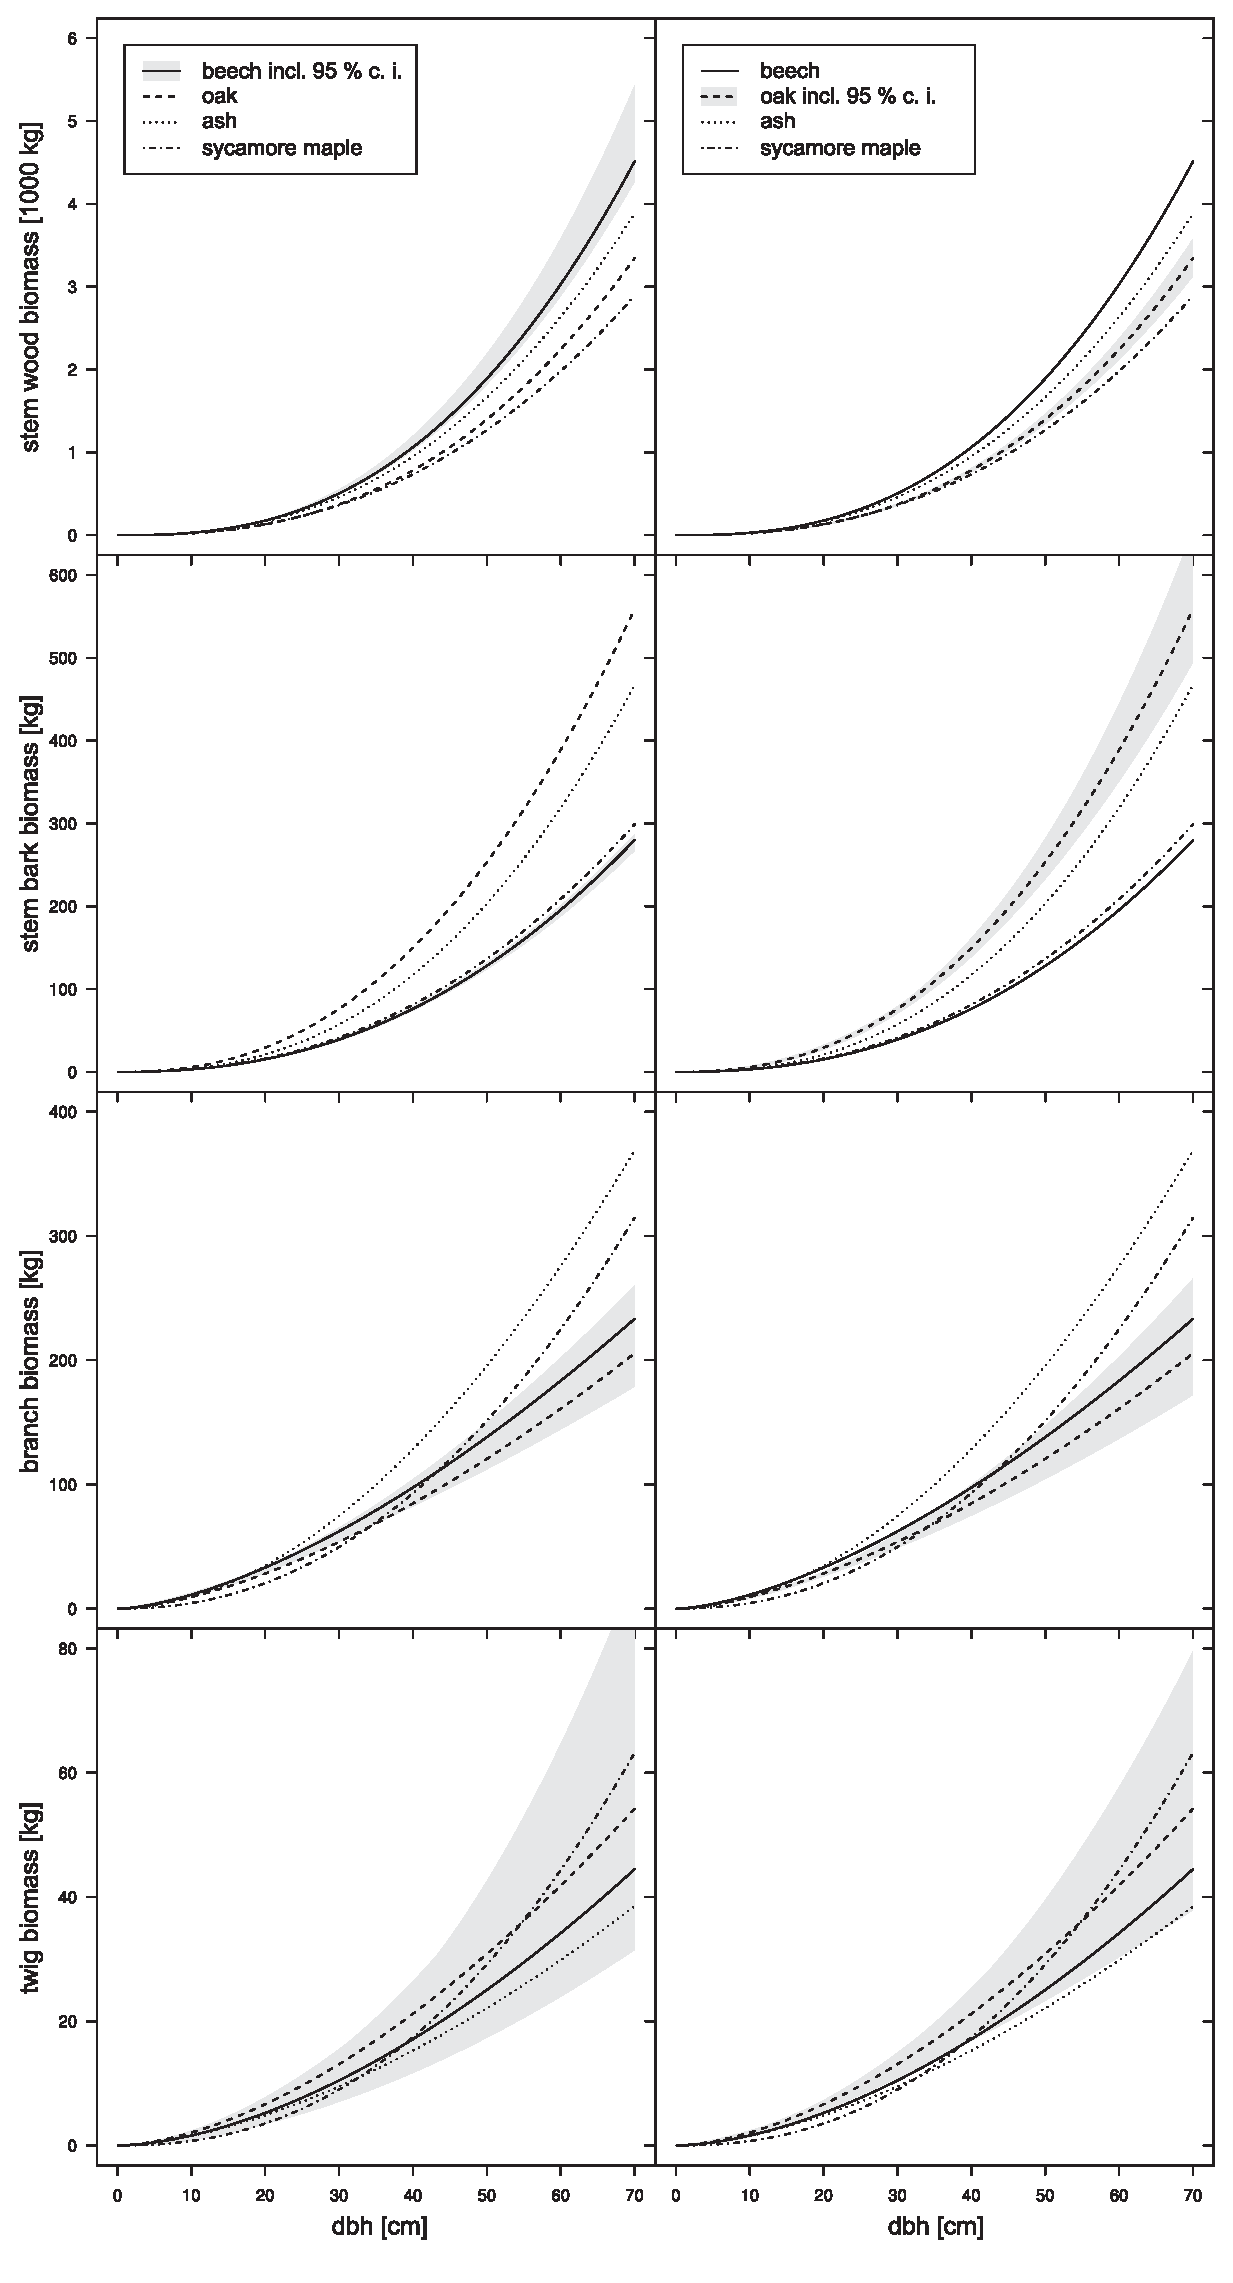
\includegraphics[width=0.75\textwidth]{Grafiken/bm/Fig_2_Regression_curves.eps}
	\caption{Regression of the biomass functions for European beech, oak, ash and sycamore over dbh. The left column includes a 95 \% confidence interval for the European beech regression function. The right column shows the same regression functions including a 95 \% confidence interval for the oak function.}
	\label{fig:bm:fig2}
\end{figure}

A comparison of the biomass models should show whether separate biomass functions for sycamore and ash are necessary. For this purpose confidence intervals were generated for the European beech and oak functions (Figure \ref{fig:bm:fig2}). We chose the 2-parametric functions with dbh as only descriptive variable for the model comparison. For stem wood there was no overlap across the whole spectrum of dbh. The curves of the stem wood functions of the 4 tree species ran more or less equidistant from one-another, with the European beech stem wood function lying above those of all other species. The lower confidence limit for the European beech stem wood function lay very near to the expected value. The European beech confidence interval had therefore no overlap with the other biomass functions. Although the oak stem wood function ran between the sycamore and ash functions, there was also no overlap with the other stem wood functions because the confidence intervals were comparatively narrow.

For the bark models there were also no areas of overlap between the graphs. The bark biomass functions could be separated into 2 groups. The graph of the sycamore bark biomass function ran very near to that of European beech. Due to the relatively large data pool and the small data variance, the confidence intervals for the European beech models were very narrow so, despite the proximity on the graph, there was no overlap with the sycamore function. The bark biomass functions for ash and oak lay almost twice as high on the graph as those of European beech and sycamore. The confidence interval of the oak function was much wider than the European beech confidence interval. The distance between the oak and ash functions is, however, so large that there was no overlap between the two.

The confidence intervals of the branch functions were altogether much wider than those of the stem wood and bark functions. The confidence interval of the European beech branch model enclosed the oak function and vice-versa. The sycamore function for branch biomass overlapped with the European beech confidence interval in the dbh range between 35 - 50 cm and with the oak function confidence interval in the range 30 - 45 cm. The graphs of the sycamore and ash branch biomass functions were, however, much steeper. Consequently there is a clear difference between the sycamore and ash branch models to the European beech and oak models.

The graphs of the 4 twig biomass models were indistinguishable over most of the value range. The confidence intervals of these functions were very asymmetric and even wider than the branch function confidence intervals. The confidence interval of the European beech function was the widest and enclosed all the other functions across the whole diameter range. The confidence interval of the oak function was slightly narrower and enclosed the European beech and sycamore functions from a dbh of ca. 40 cm and higher. The function graph of the sycamore function ran within the confidence intervals of both European beech and oak over much of the dbh value range. It was, however, much steeper than all other models. The graph of the ash function lies close under that of the European beech function. Consequently, the twig functions are mostly indistinguishable by means of the confidence interval analysis although their curvature is partially different.

The proportion of stem wood in the tree biomass increased disproportionately high with increasing dbh. For the oak functions the stem wood percentage increased sharply at first, from 56 \% by dbh 10 cm to 68 \% by dbh 20 cm. By dbh 60 cm the stem wood share of the biomass was 79 \% but did not increase much further after that. On average the stem wood share was 72 \%. The proportion of the bark biomass was more or less constant at ca. 14 \%. The share of branch as well as twig biomasses decreased with increasing dbh. The share reduced from 26 \% to 5 \% for branch and 4 \% to 1 \% for the twig biomass in the observed diameter range. The relationships between the tree fractions of the other tree species were comparable. The stem wood percentage for European beech increased from 78 \% to 89 \% in the diameter range 20 cm to 60 cm, that of sycamore from 77 \% to 81 \% and ash from 73 \% to 81 \%. For each tree species the stem wood share increases digressively and nears an asymptote. Above a dbh of ca. 60 cm the stem wood share in the tree species studied did not change much. The share of bark in the total biomass for European beech (6 \%) sycamore (9 \%), and ash (10 \%) remained relatively constant. The share of biomasses in branches and twigs thus also decreased with increasing dbh for those 3 tree species.

\begin{figure}
	\center
	\includegraphics[width=0.75\textwidth]{Grafiken/bm/Fig_3_Fraction_Biomass.eps}
	\caption{Biomass of the tree fractions in absolute scale (left) and relative to the total aboveground biomass (right) over dbh for oak.}
	\label{fig:bm:fig3}
\end{figure}

%%----------------------%%
%% Sensitivity analysis %%
%%----------------------%%
\subsection{Sensitivity analysis}
\label{subsec:bm:results:sensitivity}

In order to assess the magnitude of the effect that different biomass functions can have on results at the stand level, real and simulated test stands were used (Tables \ref{tab:bm:tab2} and \ref{tab:bm:tab4}). The sum of the total aboveground biomasses for all trees in these stands was firstly calculated with the tree species specific biomass functions. Then, secondly, the sum of the total aboveground biomasses was again calculated using only the oak biomass functions for estimating biomasses of sycamore and ash trees. The full tree biomass at the stand level for the first test stand (proportion European beech: 75 \%) was calculated to be ca. 200 t ha$^{-1}$ when using tree specific biomass functions. Using oak biomass functions for sycamore and ash led to a 4 \% overestimation of the stand biomass (ca. 7 t ha-1). The difference between the two calculation methods increased steadily with a decreasing proportion of European beech, reaching a maximum overestimation of 11 \% (21 t ha$^{-1}$) for a stand with an equal tree species mixture. If the proportion of European beech was held constant, then the difference of the total aboveground biomass on stand level increased with a decreasing ash percentage in the stand. In every case the estimated total biomass at the stand level was lower when separate, species specific, biomass functions were used.

\begin{table}[]
	\centering
	\caption{Sum of total aboveground biomass on stand level for stands with differing share of species. The biomass is calculated with distinct tree species specific biomass functions and also with oak biomass functions for ash and sycamore.}
	\label{tab:bm:tab4}
	\begin{tabular}{cccccc}
		\cline{1-3} \cline{5-6}
		\multicolumn{3}{c}{share {[}\%{]}}                                        &  & \multicolumn{2}{c}{total aboveground biomass {[}t ha$^{-1}${]}}                                                                                  \\ \cline{1-3} \cline{5-6} 
		\begin{tabular}[c]{@{}c@{}}European\\ beech\end{tabular} & ash & sycamore &  & \begin{tabular}[c]{@{}c@{}}tree specific\\ functions\end{tabular} & \begin{tabular}[c]{@{}c@{}}oak functions for\\ ash and sycamore\end{tabular} \\ \cline{1-3} \cline{5-6} 
		75                                                       & 12  & 12       &  & 199.4                                                             & 206.8                                                                        \\
		68                                                       & 25  & 7$^*$    &  & 201.6                                                             & 208.6                                                                        \\
		68                                                       & 16  & 16       &  & 199.0                                                             & 210.1                                                                        \\
		68                                                       & 7   & 25       &  & 194.5                                                             & 206.9                                                                        \\
		50                                                       & 25  & 25       &  & 197.3                                                             & 213.1                                                                        \\
		33                                                       & 33  & 33       &  & 188.1                                                             & 208.8                                                                        \\ \cline{1-3} \cline{5-6}
		\multicolumn{6}{l}{*Original test site (Table \ref{tab:bm:tab2})}
	\end{tabular}
\end{table}

%%-------------------%%
%% Nutrient contents %%
%%-------------------%%
\subsection{Nutrient contents}
\label{subsec:bm:results:nutrients}

In our analysis, the nutrient contents differed particularly between the tree species. In order to examine significant differences, we performed a parametric one-way analysis of variance for each nutrient and fraction combination with 5 \% significance level. The mean nutrients contents are listed in Table \ref{tab:bm:tab5}. All of the nutrient content data in the fraction and species groups were approximately normally distributed. For this, simple arithmetic group means are sufficient for data description and model building. This mean nutrients contents allows the tree and fraction specific calculation of the nutrients by multiplying its biomass with the respective element content from Table \ref{tab:bm:tab5}.

% Please add the following required packages to your document preamble:
% \usepackage{multirow}
\begin{table}[]
	\centering
	\caption{Group mean and standard deviation of nutrient content [g kg$^{-1}$] for the tree species European beech, oak, ash and sycamore. N: Observed number of trees.}
	\label{tab:bm:tab5}
	\begin{tabular}{ccccccccc}
		\hline
		spec.                                                                        & frac.                                                                & Ca           & Mg           & K            & C             & N            & P            & S            \\ \hline
		\multirow{8}{*}{\begin{tabular}[c]{@{}c@{}}oak\\ N=8\end{tabular}}           & \multirow{2}{*}{\begin{tabular}[c]{@{}c@{}}stem\\ wood\end{tabular}} & 0.729        & 0.100        & 1.131        & 495.898       & 1.895        & 0.087        & 0.126        \\
		&                                                                      & ($\pm$0.592) & ($\pm$0.090) & ($\pm$0.362) & ($\pm$6.515)  & ($\pm$0.736) & ($\pm$0.060) & ($\pm$0.038) \\
		& \multirow{2}{*}{bark}                                                & 26.350       & 0.768        & 2.363        & 484.346       & 6.518        & 0.276        & 0.622        \\
		&                                                                      & ($\pm$6.787) & ($\pm$0.401) & ($\pm$0.789) & ($\pm$45.123) & ($\pm$1.602) & ($\pm$0.090) & ($\pm$0.237) \\
		& \multirow{2}{*}{branch}                                              & 6.347        & 0.522        & 1.954        & 492.667       & 5.165        & 0.323        & 0.333        \\
		&                                                                      & ($\pm$2.882) & ($\pm$0.169) & ($\pm$0.223) & ($\pm$5.918)  & ($\pm$1.362) & ($\pm$0.091) & ($\pm$0.115) \\
		& \multirow{2}{*}{twig}                                                & 7.368        & 0.813        & 3.050        & 504.286       & 10.531       & 0.769        & 0.621        \\
		&                                                                      & ($\pm$2.727) & ($\pm$0.379) & ($\pm$0.395) & ($\pm$7.683)  & ($\pm$1.285) & ($\pm$0.089) & ($\pm$0.103) \\ \hline
		\multirow{8}{*}{\begin{tabular}[c]{@{}c@{}}beech\\ N=18\end{tabular}}        & \multirow{2}{*}{\begin{tabular}[c]{@{}c@{}}stem\\ wood\end{tabular}} & 0.968        & 0.302        & 1.135        & 493.686       & 1.492        & 0.100        & 0.091        \\
		&                                                                      & ($\pm$0.156) & ($\pm$0.132) & ($\pm$0.248) & ($\pm$6.100)  & ($\pm$0.520) & ($\pm$0.056) & ($\pm$0.016) \\
		& \multirow{2}{*}{bark}                                                & 22.738       & 0.517        & 2.351        & 487.684       & 6.855        & 0.351        & 0.331        \\
		&                                                                      & ($\pm$7.651) & ($\pm$0.191) & ($\pm$0.413) & ($\pm$22.248) & ($\pm$1.370) & ($\pm$0.093) & ($\pm$0.053) \\
		& \multirow{2}{*}{branch}                                              & 3.150        & 0.371        & 1.559        & 493.113       & 2.805        & 0.243        & 0.148        \\
		&                                                                      & ($\pm$1.536) & ($\pm$0.140) & ($\pm$0.309) & ($\pm$7.705)  & ($\pm$0.520) & ($\pm$0.124) & ($\pm$0.019) \\
		& \multirow{2}{*}{twig}                                                & 6.883        & 0.524        & 2.989        & 508.817       & 8.427        & 0.791        & 0.479        \\
		&                                                                      & ($\pm$2.839) & ($\pm$0.266) & ($\pm$0.569) & ($\pm$8.408)  & ($\pm$1.039) & ($\pm$0.297) & ($\pm$0.054) \\ \hline
		\multirow{8}{*}{\begin{tabular}[c]{@{}c@{}}ash\\ N=37\end{tabular}}          & \multirow{2}{*}{\begin{tabular}[c]{@{}c@{}}stem\\ wood\end{tabular}} & 0.823        & 0.193        & 1.654        & 493.495       & 1.448        & 0.092        & 0.113        \\
		&                                                                      & ($\pm$0.148) & ($\pm$0.08)  & ($\pm$0.313) & ($\pm$5.497)  & ($\pm$0.342) & ($\pm$0.036) & ($\pm$0.044) \\
		& \multirow{2}{*}{bark}                                                & 25.505       & 0.657        & 5.067        & 477.649       & 5.312        & 0.291        & 0.469        \\
		&                                                                      & ($\pm$7.428) & ($\pm$0.165) & ($\pm$1.397) & ($\pm$10.354) & ($\pm$0.644) & ($\pm$0.065) & ($\pm$0.071) \\
		& \multirow{2}{*}{branch}                                              & 4.815        & 0.319        & 2.524        & 492.675       & 2.988        & 0.228        & 0.245        \\
		&                                                                      & ($\pm$2.138) & ($\pm$0.079) & ($\pm$0.521) & ($\pm$5.58)   & ($\pm$0.647) & ($\pm$0.075) & ($\pm$0.061) \\
		& \multirow{2}{*}{twig}                                                & 8.691        & 0.83         & 6.344        & 491.191       & 8.359        & 0.769        & 0.73         \\
		&                                                                      & ($\pm$1.689) & ($\pm$0.202) & ($\pm$0.775) & ($\pm$5.982)  & ($\pm$1.175) & ($\pm$0.202) & ($\pm$0.091) \\ \hline
		\multirow{8}{*}{\begin{tabular}[c]{@{}c@{}}syca-\\ more\\ N=25\end{tabular}} & \multirow{2}{*}{\begin{tabular}[c]{@{}c@{}}stem\\ wood\end{tabular}} & 1.068        & 0.322        & 1.403        & 497.572       & 1.467        & 0.111        & 0.118        \\
		&                                                                      & ($\pm$0.26)  & ($\pm$0.129) & ($\pm$0.268) & ($\pm$3.725)  & ($\pm$0.186) & ($\pm$0.021) & ($\pm$0.021) \\
		& \multirow{2}{*}{bark}                                                & 25.184       & 0.861        & 3.784        & 474.982       & 7.737        & 0.57         & 0.772        \\
		&                                                                      & ($\pm$7.479) & ($\pm$0.21)  & ($\pm$1.027) & ($\pm$10.544) & ($\pm$1.502) & ($\pm$0.144) & ($\pm$0.134) \\
		& \multirow{2}{*}{branch}                                              & 4.089        & 0.491        & 2.394        & 493.285       & 3.403        & 0.318        & 0.283        \\
		&                                                                      & ($\pm$1.673) & ($\pm$0.122) & ($\pm$0.335) & ($\pm$4.084)  & ($\pm$0.654) & ($\pm$0.068) & ($\pm$0.059) \\
		& \multirow{2}{*}{twig}                                                & 9.668        & 0.815        & 3.889        & 495.799       & 9.948        & 0.898        & 0.709        \\
		&                                                                      & ($\pm$3.011) & ($\pm$0.227) & ($\pm$0.79)  & ($\pm$6.299)  & ($\pm$2.602) & ($\pm$0.268) & ($\pm$0.137) \\ \hline
	\end{tabular}
\end{table}

With ca. 500 g kg$^{-1}$ (dry biomass) in stem wood, as well as in bark, carbon has the greatest share of any element content in the entire dry weight. The average carbon content lies between 475 g kg$^{-1}$ and 509 g kg$^{-1}$, with slight differences between the tree species and fractions. In the stem wood sycamore differs significantly from beech while the carbon contents of other combinations do not differ significantly. In the bark fraction, ash and sycamore differ significantly from oak and beech. For sycamore and ash, the carbon content in the stem bark is a little lower than in the stem wood. The average nutrient contents, with the exception of a few calcium contents in the branches of sycamore and ash, were < 25 g kg-1. With few exceptions, the content of the various nutrients in wood can be ranked as follows: N > K > Ca > Mg > P = S. Ash has the largest potassium content (1.65 g kg$^{-1}$) of all 4 tree species. The potassium content in ash is throughout significantly higher than in all other examined species. In terms of the magnesium content, the trees can be separated into two groups. The mean content is significantly higher for sycamore and European beech than for oak and ash. Generally, the nutrient contents in bark are between 3 (N, P and K) and 25 (Ca) times higher than in wood. The concentrations of nitrogen, phosphor and sulfur in sycamore bark are always significantly higher than those of European beech and than those in the bark of oak and ash. The bark of ash has significantly lower nitrogen concentrations than the other species but higher potassium content.

%%%%%%%%%%%%%%%%
%% Discussion %%
%%%%%%%%%%%%%%%%
\section{Discussion}
\label{sec:bm:discussion}

%%-------------------%%
%% Biomass functions %%
%%-------------------%%
\subsection{Biomass functions}
\label{subsec:bm:discussion:bm_functions}

Biomass functions.

%%----------------------%%
%% Sensitivity analysis %%
%%----------------------%%
\subsection{Sensitivity analysis}
\label{subsec:bm:discussion:sensitivity}

Sensitivity.

%%-------------------%%
%% Nutrient contents %%
%%-------------------%%
\subsection{Nutrient contents}
\label{subsec:bm:discussion:nutrients}

Nutrients.

%%%%%%%%%%%%%%%%%
%% Conclusions %%
%%%%%%%%%%%%%%%%%
\section{Conclusions}
\label{sec:bm:conclusions}

Conclusion

%%%%%%%%%%%%%%%%%%%%%%
%% Acknowledgements %%
%%%%%%%%%%%%%%%%%%%%%%
\section*{Acknowledgements}
\label{sec:bm:acknowledgements}
We would like to thank the German Science Foundation (DFG) for financial support of this study (Sachbeihilfe SA 415/5-1) and Dr. B�ckmann of the Lower Saxony Forest Planning Office for his kind provision of the inventory data.
Moreover, we would like to thank two anonymous reviewers for their helpful comments.

	\clearpage
	\newpage
	\mbox{}
	\pagebreak
	\thispagestyle{empty}
	\chapter{Modelling the economically viable wood in the crown of European beech trees}
\label{chap:beech_crowns}
{\large Kai Husmann$^1$ - Bernhard M�hring$^1$}\\

\vspace{3cm}
\noindent
$^1$Department of Forest Economics and Forest Management,\\ University of G�ttingen, B�sgenweg 3, 37077 G�ttingen, Germany \\

\vspace{\fill}
\noindent
Published in:\\
Forest Policy and Economics.\\(DOI: 10.1016/j.forpol.2017.01.009)


\cleardoublepage
%%%%%%%%%%%%%%
%% Abstract %%
%%%%%%%%%%%%%%
\section*{Abstract}
\label{chap:beech_crowns:Abstract}
Long-term forest development programs in Germany aim on an increase of close-to-nature broadleaf forest stands. This means that the economic importance of European beech is expected to increase. The economic potential of a tree basically consists of the stem as well as the economically viable wood volume in the crown. Due to the high morphological variability of European beech crowns, taper models are often not satisfactory for predicting the economically viable wood volume arising from crowns. Prediction models with a higher precision are recently still lacking. Aim of this study is thus the development of prediction model for the economically viable crown wood volume of European beech trees.

We determined the distribution of the wood volume in the crown over the branch diameters using the multistage "randomized branch sampling" method (RBS). The tree-specific wood volume distribution on the branch diameters were used to cluster all sampled trees into 3 groups. Additionally, we developed a method able to distinguish between economically viable and unviable crown branches. Basing on the RBS measurements as well as revenues and processing costs, we modeled the economically viable wood volume from the crown for each tree. To calculate the wood volume under bark, we parameterized a bark thickness function from disk samples of the trees.

We showed that the European beech crowns could be clustered into 3 groups differing in their wood volume distribution. The economically viable wood volume in the crown significantly depended on this grouping parameter as well as diameter at breast height (DBH). By contrast, the total amount of wood in the crown only depended on DBH. The differing viable wood volumes in the crowns were thus explained by different wood distributions and not by differing total crown wood volume. To make the results applicable in practice forestry, the modeling results were used to develop a regression formula able to predict the economically viable wood volume in the crown depending on the DBH and the crown type. As the crown type can also be predicted via measurable tree covariates, the regression model of the viable wood volume in the crown can be used as a support tool for the management of European beech stands. Sensitivity analysis quantifies how harvest revenues and costs translate into different viable tree volume.

\subsection*{Keywords}
Economically optimal wood cut, Crown morphology, European beech, viable crown wood, wood allocation, forest management

\subsection*{Highlights}
\begin{itemize}
\item Morphological measurements of 163 European beech tree crowns via "RBS" method.
\item Distinguishing the economically viable from the whole crown wood.
\item Categorization of European beech crowns into morphological types.
\item Development of a viable crown timber prediction model for forest management.
\end{itemize}

%%%%%%%%%%%%%%%%%%
%% Introduction %%
%%%%%%%%%%%%%%%%%%
\section{Introduction}
\label{sec:beech_crowns:Introduction}
Although European beech (Fagus sylvatica L.) forests have been identified as the dominant forest communities in the potential natural vegetation of Germany \citep{fanc_2010}, with 1,680,072 ha, they currently only account for 15 \% of Germany?s forest stand cover \citep{ti_2014b}. Long-term ecological forest development programs result in a general increase in deciduous tree species with a focus on European beech \citep{mfacp_2004}. The economic importance of European beech will thus further increase.

Traditionally the objective of European beech management is to maximize valuable stem wood \citep{nagel_2008}. Especially under the perspective of modern utilization methods like bio-economics \citep{hildebrandt_2014} and the increasing demand for fuel wood \citep{mantau_2012}, the economic importance of smaller branches of European beech is expected to increase. Thus a large proportion of the economic potential lies in smaller branches. Under certain conditions, further economic potential can be found in the tree stump and foliage \citep{miettinen_2014}. For a suitable management of European beech stands, it is necessary to assess the economically viable wood cut fully \citep{mohring_1997}. Therefore, as well as predicting the wood from the sympodial stem, it is also necessary to predict the economically viable wood cut in the sympodial crown. In the complex crowns of broadleaf trees, the economically viable wood can be substantially smaller than the whole wood volume. For this purpose, a model able to distinguish the economically viable wood volume from the whole wood volume in the crown is needed. For the stem volume prediction, there are many different and sophisticated tariff and other functions available. Cubic taper models exist, providing an adequate prediction of the economic potential of coniferous trees and the stems of deciduous trees \citep{kuzelka_2012}. However, those taper functions do not account for the complex sympodial form above the crown base of broadleaf tree species where the wood volume is not allocated around a throughout stem axis. They are therefore imprecise in predicting the wood volume arising above the crown base. They are usually calibrated for a minimum small-end diameter threshold of 7 cm. This small-end diameter can lack economic interpretation.

The aim of this study is to develop a parametric, practically usable prediction model of the economically viable wood volume in the crown of European beech trees. For this purpose, 163 beech trees were felled. Using the multistage "Randomized Branch Sampling" (RBS) method \citep{gaffrey_1999}, a sound sample of branches was measured from each tree. The measurements were taken to examine the tree individual distribution of the wood volume in the crown on the crown branches. To develop tree individual morphological covariates, the sampled trees were clustered into groups with differing wood volume distribution. A multinomial regression model enables the prediction of this covariate via measurable tree attributes. We additionally developed a model, which predicts the viable wood volume from the measured wood volume distribution. This viable wood volume does not depend on freely selected but on economically justified small-end diameters. We developed a method to classify economically viable and unviable branches in European beech crowns via a break-even analysis. Then only the wood volumes of viable branches were estimated via RBS. The modeled economically viable wood volume thus depends on the size of the tree and the volume distribution in the crown. To calculate the wood volume under bark, we parameterized a new bark thickness function from disk samples of the trees.
To make the results applicable in forest practice, we performed a regression analysis with the modeled economically viable wood volume and further tree covariates. To ensure the applicability, we only used practically measurable tree attributes. The regression model represents a new approach for modeling the economic potential of European beech crowns and therefore a novel decision support tool for forest management operations.

%%%%%%%%%%%%%%%%%%%%%%%%%%%
%% Materials and Methods %%
%%%%%%%%%%%%%%%%%%%%%%%%%%%
\section{Materials and Methods}
\label{sec:beech_crowns:methods}
The dataset for this study comprised measurements from a destructive sample of 163 European beech trees sampled using the multistage RBS method \citep{gaffrey_1999, jessen_1955}. These data were compiled from 2 existing databases at the Northwest German Forest Research Station and the Baden-W�rttemberg Forest Research Centre.
%%-------------------------------------%%
%% Data sampling and sample processing %%
%%-------------------------------------%%
\subsection{Selection of trees}
\label{subsec:beech_crowns:methods:tree_selection}
The data were collected during 2009 and 2014. Altogether 163 trees were destructively sampled. In order to cover as many growth zones as possible, the sample plots were distributed throughout Germany (Figure \ref{fig:beech_crowns:fig1}). To ensure representation of the entire relevant diameter range, we chose up to 3 forest sites with different stand ages within these growth zones. All selected sites were high forests under standard management regimes. Depending on the area size of the plot, 2 - 4 sample trees were selected. In addition to the morphological measurements via RBS, DBH and tree height were measured (Table \ref{tab:beech_crowns:tab1}).

\begin{figure}
	\center
	\includegraphics[width=0.5\textwidth]{Grafiken/beech_crowns/Fig_1_plot_locations.eps}
	\caption{Sample site locations. Source of the background map: \citet{facg_2014}.}
	\label{fig:beech_crowns:fig1}
\end{figure}

\begin{table}[]
	\centering
	\caption{Summary statistics of the sampled trees. The sample size was 163.}
	\label{tab:beech_crowns:tab1}
	\begin{tabular}{cccc}
		\hline
		             &DBH [cm]        & height [m]  & age [a] \\ \hline
		min          & 8.0            & 13.1        & 21      \\
		mean         & 35.4           & 25.3        & 85      \\
		median       & 34.8           & 26.0        & 80      \\
		max          & 78.3           & 38.5        & 180     \\ \hline
	\end{tabular}
\end{table}

%%--------------------%%
%% Selection of disks %%
%%--------------------%%
\subsection{Selection of disks}
\label{subsec:beech_crowns:methods:disk_selection}

To subtract bark from the wood volume, stem and branch disks for bark thickness measurement were taken from 37 trees of the NW-FVA study (Table \ref{tab:beech_crowns:tab2}). Up to 6 disks were randomly selected using the importance sampling method \citep{Gregoire_2008}. The proxy function, which is necessary for calculation of the sampling probability, was derived by the volume distribution of the branch diameters over the approximated tree height (which were both measured for volume estimation via RBS anyway). The selection probability of the disks was thus proportional to their disk diameter. Diameter and the bark thickness of the disks were measured at 4 directions of the selected disks directly after extraction.

\begin{table}[]
	\centering
	\caption{Summary statistics of disks for bark thickness measurements.}
	\label{tab:beech_crowns:tab2}
	\begin{tabular}{ccccccccccc}
		\cline{3-6} \cline{8-11}
		&  & \multicolumn{4}{c}{single bark thickness {[}mm{]}} &  & \multicolumn{4}{c}{disk diameter over bark {[}cm{]}} \\ \cline{1-1} \cline{3-6} \cline{8-11} 
		N   &  & min        & mean       & median       & max       &  & min        & mean        & median       & max        \\ \cline{1-1} \cline{3-6} \cline{8-11} 
		149 &  & 0.6        & 3.0        & 2.4          & 9.0       &  & 1.0        & 18.0        & 12.0         & 64.2       \\ \cline{1-1} \cline{3-6} \cline{8-11} 
	\end{tabular}
\end{table}

%%-----------------------%%
%% Selection of branches %%
%%-----------------------%%
\subsection{Selection of branches}
\label{subsec:beech_crowns:methods:branch_selection}
The estimation of the wood volume in the crown was based on the RBS method of multistage probability sampling. RBS is an unbiased method of probability sampling used for estimating specific tree parameters by measurable auxiliary variables \citep{jessen_1955,gaffrey_1999}. In our application, RBS enables estimation of the wood volume in the crown or in specific parts of the crown by measuring only a sample of branch segments instead of measuring all branch segments in the crown. Only relatively few measurements of branch diameters and branch segment lengths have to be taken for an accurate estimate of the whole wood volume in the crown or the wood volume of specific crown parts.

RBS is based on the knowledge of the conditional probability $q_{lj}$ of choosing the $j$-th out of n "branches" at a "node" $l$ in the crown instead of choosing another branch of this node. The probability $q_{lj}$ can be calculated by an auxiliary variable instead of the (complicated measurable) target variable itself \citep{gregoire_1995,Gregoire_2008,valentine_1984}. Instead of measuring the volume of all branches at a node, in our case, we only had to measure the base diameters $d_{lj}$ of the branches to calculate $q_{lj}$ and the volume of one branch. As \citet{west_1999} examined an allometric coefficient of 2.67 between branch volume and branch base diameter, the branch base diameter to the power of 2.67 is expected to provide efficient estimates. In our study, the conditional probability has been selected to be

\begin{equation}
	\label{eq:beech_crowns:eq1}
	q_{lj}(d)=d_{lj}^{2.67}/ \sum_{j=1}^{n_l} d_{lj}^{2.67}
\end{equation}

Thus once all branch base diameters $d_{li}$ at a node were recorded, one of the branches can be randomly chosen with probability $q_{lj}$. Only the "segment" volume of this chosen branch has to be measured, where a "segment" is defined as the part of the branch between 2 nodes \citep{Gregoire_2008}. We chose the formula for a conical frustum (Equation \ref{eq:beech_crowns:eq2}) to calculate the segment volume $v_{lj}$ via the branch base diameter $d_{lj}$, the base diameter at the following node $d_{lj+1}$ and the segment length $h_{lj}$. The volume of the following node $d_{lj+1}$ was also measured and added to the segment volume $v_{lj}$.

\begin{equation}
	\label{eq:beech_crowns:eq2}
	v_\mathit{lj}=\frac{h_{lj}\pi}{12}\left(d_{lj}^2+d_{lj}d_{{lj}+1}+d_{{lj}+1}^2\right)
\end{equation}

The crown base, which is the height where the throughout stem ends and the sympodial crown starts, represented the first node of the RBS procedure. To have a measurable criterion, we defined the crown base to be the tree height where a branch base diameter was > 1/5 of the stem diameter at that height. A whole RBS path thus consisted of a succession of randomly selected branch segments from the crown base up to one shoot bud. Along the path all branch base diameters and all segment volumes were measured. In order to get an idea of the variation, 3 random and distinct RBS paths were obtained for each of the 163 sampled trees.

%%--------------------------------------------------------%%
%% Estimation of wood volume in the stem and in the crown %%
%%--------------------------------------------------------%%
\subsection{Estimation of wood volume in the stem and in the crown}
\label{subsec:beech_crowns:methods:crown_vol_est}
The calculation method for the point estimates of the volumes as well as for the estimated variance is described in the literature \citep[e. g.][]{Gregoire_2008}. The stem form was assessed by section-wise diameter measurements at certain tree heights up to the crown base. The sum of these section volumes, also calculated by the conical frustum formula (Equation 2), gave the whole stem volume from the ground up to the crown base.

%%----------------------------------------------%%
%% Economically viable wood volume in the crown %%
%%----------------------------------------------%%
\subsection{Economically viable wood volume in the crown}
\label{subsec:beech_crowns:methods:viable}

%%++++++++++++++++++++++++++++%%
%% Crown type differentiation %%
%%++++++++++++++++++++++++++++%%
\subsubsection{Crown type differentiation}
\label{subsubsec:beech_crowns:methods:viable:crown_types}
To calculate the volume distribution according to the branch diameters in individual tree crowns, the cumulative wood volume amount $\hat{V}_i(d)$ in the crown was calculated from the crown base up to each recorded branch base diameter $(d)$ along each RBS path. This distribution was normalized by dividing the predicted cumulative crown volume below $\hat{V}_i(d)$ [m3] by the whole wood volume from the crown $\hat{V}_i(0)$ [m3] (Equation \ref{eq:beech_crowns:eq3}) and by dividing the base diameter of every branch $d_{ij}$ by the maximum diameter found $d_{max}$. $F(d)$ thus denotes the wood volume amount over branch diameter in the crown.

\begin{equation}
\label{eq:beech_crowns:eq3}
F\left(d\right)=\frac{{\widehat V}_i\left(d\right)}{\widehat V}
\end{equation}

The diameter where half of the wood volume amount was located above (below respectively) was interpreted as the median branch diameter of a tree crown. This median volume branch diameter $F(d_{0.5})$ was easily interpolated from the generated diameter distribution for every RBS path, where $d_{0.5}$ denotes the branch diameter for which $F(d_{0.5})=0.5*F(d_{max})$. The same appears for the lower $F(d_{0.25})$ and upper quantile $F(d_{0.75})$. The curve trend of $F(d)$ over branch diameter thus indicates whether most of the wood volume is located in relatively small or in larger branches. Generally, there were 3 types of volume distribution in the data (Fig. \ref{fig:beech_crowns:fig2}). The first type showed a high share of volume in relatively small branch dimensions (left). The median branch diameter of these trees was close to the lower quantile. In the balanced type (center), half of the wood volume was found above a branch diameter that was approximately half the size of the largest diameter of the respective tree. In the third type (right), major part of wood volume was allocated in the larger branch diameter range. The median diameter was close to the upper quantile.

\begin{figure}
	\center
	\includegraphics[width=1\textwidth]{Grafiken/beech_crowns/Fig_2_relative_volume_amount.eps}
	\caption{Cumulative crown wood volume over relative branch diameter for 3 exemplary trees. For each tree all 3 RBS paths are displayed. The diameters where half of the timber volume is located above, respective below (the median relative branch diameter) are marked by vertical lines.}
	\label{fig:beech_crowns:fig2}
\end{figure}

As there were 3 paths per tree, the tree individual median diameter was calculated by the median of the 3 median branch diameters. The lower and upper quartiles were created in the same way. We thus generated 3 tree individual continuous variables. These enabled a clustering of the trees into 3 crown types which differ in their wood volume amount. As the crown types based on the volume distribution in the crowns, they should represent groups with different economically viable wood volumes. We chose the "k-means" cluster algorithm \citep{r_core_team_2016}, which minimizes the within-cluster Euclidean distance among observations and group means by the sum-of-squares method \citep{wagstaff_2001}, to cluster the data into 3 morphological crown types.

The median tree diameter as well as the quantile tree diameters are not measurable in practice. To differentiate a beach crown into 1 of the 3 mentioned groups in forest management, it is thus necessary to predict the crown type by other tree attributes. A multinomial logistic regression method \citep{hutcheson_2008} was parameterized to predict the crown type clusters from practically measurable morphological tree variables $x_i$ (equation 4). In this case, the $x_i$ are the DBH, the tree height, the tree height at crown base and the ratio of the base diameters at crown base. The ratios of the branch diameters at crown base were calculated by dividing the 2nd largest base diameter at the crown base by the respective largest branch diameter.

We fitted a log odd model with $J=3$ categories to a probability function which predicts the probability that an individual tree is belonging to a crown type category $j$ rather than to the reference category $j^{'}= 1$ by $i=4$ variables.

\begin{equation}
\label{eq:beech_crowns:eq4}
\operatorname{log}\left(\frac{P\left(Y=j\right)}{P\left(Y=j^{'}\right)}\right)=\beta_{j0}+\beta_{j1}x_{1}+\beta_{j2}x_{2}+\dots+\beta_{ji}x_{i}
\end{equation}

The probability of an individual to belong to group j in relation to the reference is therefore calculated as

\begin{equation*}
P\left(Y=j\right)=\frac{\operatorname{exp}\left(\beta_{0}+\beta_{j1}x_{1}+\beta_{j2}x_{2}+\dots+\beta_{jk}x_{k}\right)}{1+\operatorname{exp}\left(\beta_{0}+\beta_{j1}x_1+\beta_{j2}x_{2}+\dots+\beta_{jk}x_{k}\right)}=\frac{exp(\boldsymbol{x}_i^{'}\boldsymbol{\beta}_j)}{1+exp(\boldsymbol{x}_i^{'}\boldsymbol{\beta}_j)}
\end{equation*}

and the probability of an individual to belong to group j considering all groups calculates as

\begin{equation*}
P\left(Y=j\right)=\frac{exp(\boldsymbol{x}_i^{'}\boldsymbol{\beta}_j)}{1+\sum_{s=1,s\neq j'}^{J} exp(\boldsymbol{x}_i^{'}\boldsymbol{\beta}_s)}
\end{equation*}

where crown type 1 represented the reference category $j^{'}$. The model was fitted with the R package "NNET" \citep{venables_2002}. The significance of a variable was examined by linear discriminant analysis. For model quality testing we predicted the crown type with our model and compared the result with the actual crown classification by the k-means analysis. This classification was performed by a leave-one-out cross-validation \citep[R package "MASS";][]{venables_2002} and an in-sample reclassification.
%%++++++++++++++++++++++++++++++++++++++++++++++++++++++++++++%%
%% Modelling the economically viable wood volume in the crown %%
%%++++++++++++++++++++++++++++++++++++++++++++++++++++++++++++%%
\subsubsection{Modelling the economically viable wood volume in the crown}
\label{subsubsec:beech_crowns:methods:viable:econ_viable}
As biasedness of the point and the variance estimate do not depend on the number of stages, RBS also allows the volume estimation of specific parts in the crown \citep{cancino_2005}. We used this property to estimate the tree individual viable wood volume in the crown only. For this, we programmed a model that distinguished the economically viable from economically unviable branches in the RBS sample (Algorithm 1). After running the algorithm, only the economically viable branches were then used to estimate the wood volume via the RBS method. The predicted wood volume after application of the separation algorithm thus reflected the economically viable wood volume in the crown.

\RestyleAlgo{boxruled}
\begin{algorithm}[H]
	initialization of processing $costs$ and $revenue$ by the user\\
	aggregation of the RBS $knots$ and $branch$ $segments$ into $structures$ \\
	\hfill \\
	\For{i in (1 : $N_{paths}$)}{
		\For{j in (1 : $N_{structures}$)}{
			\eIf{volume of $structure_{ij}*revenue > processing$ costs}
			{\eIf{$economical$ $viability$ $of$ $structure_{ij-1}$==TRUE}
				{$economical$ $viability$ $of$ $structure_{ij} \leftarrow TRUE$ \\
					$small-end$ $diameter_j$ $\leftarrow$ $end$ $diameter$ $of$ $structure_{ij}$}{
					\eIf{volume of $structure_{ij}*revenue > processing$ $costs*2$}
					{$economical$ $viability$ $of$ $structure_{ij} \leftarrow TRUE$ \\
						$small-end$ $diameter_j$ $\leftarrow$ $end$ $diameter$ $of$ $structure_{ij}$}
					{$economical$ $viability$ $of$ $structure_{ij} \leftarrow FALSE$}}
			}
			{$economical$ $viability$ $of$ $structure_{ij} \leftarrow FALSE$}
		}
	}
	\hfill \\
	$crown$ $timber$ $volume$ $\leftarrow$ RBS estimation of the viable structures \\
	$variance$ $\leftarrow$ RBS estimation of the viable structures\\
	$small$-$end$ $diameter$ $\leftarrow$ mean($small$-$end$ $diameter_1$, $...$, $small$-$end$ $diameter_{N_{paths}}$)
	\\
	\hfill \\
	
	\textbf{return} ($crown$ $timber$ $volume$, $variance$, $small$-$end$ $diameter$) \\
\caption{Pseudocode of the of the economically viable wood volume distinguishing model where $N_{paths}$ is the number of paths per tree (in this study always 3) and $N_{structures}$ is the number of branch structures per path.}
\label{alg:beech_crowns:alg1}
\end{algorithm}

To distinguish viable from unviable branches, each RBS node and subsequent selected branch segment were aggregated into one "branch structure". In the event that many nodes occurred in close succession (no branch segments in between), they were regarded as one large node and aggregated with the following node and branch segment to form a large branch structure.

Each of the branch structures were then, starting at the crown base, successively rated in terms of revenue and cost. The revenue was calculated by multiplying wood volume [$\text{m}^3$] (under bark) by timber price [$\text{\euro} \text{m}^{-3}$]. The cost associated with any one branch structure was assumed to be constant per processing step and was interpreted as marginal cost \citep{mohring_1997} of processing this branch structure. Whenever a branch structure had a positive marginal return, it was additionally proofed if the former branch structure was viable. If this was the case, the branch structure was labeled to be economically viable. A branch segment is thus only considered as economically viable if its piece-volume is large enough to have a positive marginal return. If a former branch structure was unviable, the processing costs doubled, because the continuation of processing thereafter would require an additional cut. Each RBS path of every crown thus had a specific break-even point \citep{starr_1975} after which further processing would result in lower marginal returns. The small-end diameter of this last viable branch structure was recorded. The model was programmed in the statistical programming language R \citep{r_core_team_2016}.

After neglecting the unviable branch structures, the tree individual viable wood volume from the crown as well as the variance were estimated by means of RBS. The final small-end diameter of an individual tree was defined as the mean of the end diameter of all 3 paths.

The model (Algorithm \ref{alg:beech_crowns:alg1}) thus needed timber price [$\text{\euro} \; \text{m}^{-3}$] (under bark) and marginal costs [$\text{\euro} \; \text{processing step}^{-1}$] as input parameters. It was parameterized with commonly used values to ensure realistic results. The revenue was set to 50 $\text{\euro} \; \text{m}^{-3}$ (under bark) to reflect the common price for industrial wood in Germany in 2016 \citep{degenhard_2016}. The fixed cost parameter was based on the European beech wages table from the forest entrepreneurs association \citep{haarhaus_2012}, which assumes an 125 \% entrepreneur fee and 19 \% value added tax. Based on the assumptions that each node occurring represented one processing step and that the costs of each were constant, the costs amounted to 0.35 $\text{\euro} \; \text{processing step}^{-1}$. The model outputs were the economically viable wood from the crown (under bark) [$\text{m}^3$] and small-end diameter [mm].

\begin{equation}
\label{eq:beech_crowns:eq5}
\begin{aligned}y&=\beta\prod_{i=1}^kx_i^{\alpha_i}\\\leftrightarrow\operatorname{log}\left(y\right)&=\operatorname{log}\left(\beta\right)+\sum_{i=1}^k\alpha_i\operatorname{log}\left(x_i\right)\end{aligned}
\end{equation}

The modeled viable wood volumes were used to parameterize an allometric growth model (Equation \ref{eq:beech_crowns:eq5}) with $k$ covariates. This parametric regression model allows forecasting of the economically viable crown wood volume by measurable covariates and is therefore easily applicable in forest management. For this purpose, sets of results, differing in their parameterization of input variables, were generated with the viable wood volume prediction model (Algorithm \ref{alg:beech_crowns:alg1}). The revenue as well as the cost input parameters were firstly set to the common parameter combination (50 $\text{\euro} \; \text{m}^{-3}$, 0.35 \euro \; $\text{step}^{-1}$) and then separately changed by 20 \%. Altogether, there were 9 result sets generated where each set of results involved 163 datasets. Because there were void datasets, whenever the algorithm assigned no viable wood volume in the crown, the data reduced to 1347 datasets. The regression analysis was composed of the covariates DBH, tree height, tree height at crown base, crown width, diameter ration at crown base and tree age as well as crown type, revenue scenario and cost scenario, which both functioned as dummy variable. The dependent variable was the modeled economically viable wood volume in the crown. The significance analysis and the model parameterization were performed by a "Generalized Linear Model" \citep[R Package "stats";][]{r_core_team_2016}. Proof of the significant impact of the covariates on $\alpha$ was not possible due to insufficient crown type 3 observations in larger DBH dimensions. The significance analysis was thus performed on $\beta$. Linearity and homoscedasticity were achieved by a Gamma distributed log-link function \citep{wood_2006}.
%%--------------------------%%
%% Allometric relationships %%
%%--------------------------%%
\subsection{Allometric relationships}
\label{subsec:beech_crowns:methods:allo}
In the metabolic scaling theory, the relationship between two plant organs ($y$ and $x$, see also Equation \ref{eq:beech_crowns:eq5}) can be described by a power law \citep{huxley_1932,niklas_1994}. This power law interprets the intraspecific relationship between plant organs for a given species. The variability of the relationship describes the strength of the allometry \citep{pretzsch_2010,west_1997}. Allometric model are thus useful to investigate the relationship between variables of economic interest and further tree attributes.

To consider the assumption of allometric regressions \citep{stumpf_2012}, we transformed the data by taking the natural logarithm. The relationships were regressed with the "standardized major axis" method \citep[R package "SMATR";][]{warton_2012}. The retransformation bias was estimated and corrected from the residual standard error of the log linear model \citep{sprugel_1983}.
%%%%%%%%%%%%%
%% Results %%
%%%%%%%%%%%%%
\section{Results}
\label{sec:beech_crowns:results}

%%------------------------------%%
%% Estimation of bark thickness %%
%%------------------------------%%
\subsection{Prediction of bark thickness}
\label{subsec:beech_crowns:results:bark}
To subtract the bark from the wood volume, models for the double bark thickness over branch diameter are necessary. The predicted double bark thickness enabled the bark subtraction from both sides of the RBS diameter measurements. The commonly used double bark thickness model of \citet{altherr_1978} was parameterized with stem and branch disks of diameters above 7 cm. As the wood volume model in this study should be able to predict smaller branches as well, parameterization of an own bark thickness model became necessary. In addition, comparison of the observed bark thickness to the predicted bark thickness with the equation by \citet{altherr_1978} revealed that application of the Altherr model would have led to an overestimation of the bark thickness. The estimated double bark thickness with the function by \citet{altherr_1978} was 1.4 mm higher than with the new parameterized function for branches with a diameter of 10 cm. For branches with diameter of 30 cm, the difference amounted to 3.1 mm.

The double bark thickness regression equation was calculated via a "Generalized Additive Mixed Model" \citep{wood_2006} using the untransformed normally distributed identity link function. A linear curve trend was found in the bark thickness model (Fig \ref{fig:beech_crowns:fig3}). There were multiple measurements in one tree (see section \ref{subsec:beech_crowns:methods:disk_selection}). To exclude regional as well as tree specific influences, the tree id was considered a random effect. As we found heteroscedasticity, we weighted our data by a power function, which was parameterized by the model residuals over the fitted values.

\begin{figure}
	\center
	\includegraphics[width=0.7\textwidth]{Grafiken/beech_crowns/Fig_3_bark_thickness.eps}
	\caption{Double bark thickness over disk diameter (over bark) and the fitted linear bark thickness model.}
	\label{fig:beech_crowns:fig3}
\end{figure}

The model (Table \ref{tab:beech_crowns:tab3}) represented a valid method for subtracting bark from both sides of every morphological RBS diameter measurement. The volume calculation after bark subtraction via RBS thus predicts the volume under bark. This was also done for the section-wise stem diameter measurements to predict the stem wood volume under bark.

\begin{table}[]
	\centering
	\caption{Summary statistics of the linear double bark thickness [mm] regression model. Independent variable is the diameter over bark [cm] (fresh).}
	\label{tab:beech_crowns:tab3}
	\begin{tabular}{ccccc}
		\hline
		variable             & coefficient & standard error & t-value & p-value          \\ \hline
		intercept            & 1.87804     & 0.25           & 7.42    & \textless2*10-16 \\
		diameter             & 0.23253     & 0.01           & 16.06   & \textless2*10-16 \\ \hline
		observations         & 149         &                &         &                  \\
		AIC                  & 565.0       &                &         &                  \\
		model range {[}cm{]} & 0 - 65      &                &         &                  \\ \hline
	\end{tabular}
\end{table}

%%----------------------------------------------%%
%% Economically viable wood volume in the crown %%
%%----------------------------------------------%%
\subsection{Economically viable wood volume in the crown}
\label{subsec:beech_crowns:results:viable}

%%++++++++++++++++++++++++++++%%
%% Crown type differentiation %%
%%++++++++++++++++++++++++++++%%
\subsubsection{Crown type differentiation}
\label{subsubsec:beech_crowns:results:viable:crown_types}
All calculated and measured crown morphology variables and tree metadata, including mean coefficient of variation for the data estimated by the RBS method, are summarized in Table \ref{tab:beech_crowns:tab4}. The crown type classification analyses were based on the median branch diameter and the branch diameter quartiles. The other tree variables were then used to parameterize a prediction model for the crown type classes.

\begin{table}[]
	\centering
	\caption{Summary statistics of all used variables, c. v. = coefficient of variation.}
	\label{tab:beech_crowns:tab4}
	\begin{tabular}{cccccccc}
		\hline
		variable                       &                            & unit     & min   & median & mean  & max    & c. v. \\ \hline
		diameter at breast height      & $DBH$                        & {[}cm{]} & 8.0   & 34.8   & 35.4  & 78.3   & -     \\
		tree height                    & $H$                          & {[}m{]}  & 13.1  & 26.0   & 25.3  & 38.5   & -     \\
		whole tree wood volume         & $V_t$                       & [$\text{m}^3$] & 0.05 & 1.46  & 2.25 & 11.70 & 0.07 \\
		crown wood volume              & $\hat{V}_i(0)$ & [$\text{m}^3$] & 0.01 & 0.64  & 1.21 & 9.20  & 0.22 \\
		tree wood volume (u. b.) & $V_{tub}$                     & [$\text{m}^3$] & 0.04 & 1.36  & 2.11 & 10.98 & 0.07 \\
		crown wood volume (u. b.)      & $V_{cub}$                    & [$\text{m}^3$] & 0.01 & 0.59  & 1.12 & 8.62  & 0.22 \\
		median branch diameter         & $F(d_{0.5})$                 & [$\text{m}^3$] & 23  & 138  & 152 & 406  & -     \\
		height at crown base           & $CB$                         & {[}m{]}  & 1.6   & 10.9   & 10.8  & 21.1   & -     \\
		diameter ratio at crown base   & $DR$                         & -        & 0.2   & 0.4    & 0.4   & 0.9    & -     \\ \hline
	\end{tabular}
\end{table}

The trees were clustered into 3 groups, where 50 trees were assigned to the first (bulk of volume in smaller branches), 69 to the second (balanced volume allocation) and 44 to the third (bulk of volume in larger branches) crown type. As median and quantile tree diameters cannot be measured practically but the model shall be applicable in forest management, the influence of measurable variables on the crown types was assessed. The influence of tree attributes on the crown type was tested by linear discriminant analysis \citep{venables_2002}, analysis of variance and deviance \citep{chambers_1992} as well as analysis of Akaike Information Criterion \citep{akaike_1981}. Only significant variables and interactions were chosen as regression parameters (Table 5). The analysis of variance revealed the significance of the diameter ratio at crown base $DR$. Deviance of the residuals (310.3 without $DR$) as well as AIC (330.0 without $DR$) were also substantially improved by this variable. Due to their high linear correlation with the significant variables, tree age and crown width were insignificant. The model is applied by plugging the coefficients of Table \ref{tab:beech_crowns:tab5} into Equation \ref{eq:beech_crowns:eq4}.

\begin{table}[]
	\centering
	\caption{Summary statistics of the multi-nominal logistic crown type prediction model with independent variables DBH [cm], tree height (H) [m], height at crown base (CB) [m] and branch diameter ratio at crown base (DR) including the results of the leave-one-out cross-validation (c.-v.) and the within-model reclassification (w.-m.).}
	\label{tab:beech_crowns:tab5}
	\begin{tabular}{clcclcc}
		\cline{3-4} \cline{6-7}
		&   & \multicolumn{2}{c}{crown type 2}   &   & \multicolumn{2}{c}{crown type 3}  \\ \cline{1-1} \cline{3-4} \cline{6-7} 
		Variable   &   & coefficient    & standard error    &   & coefficient    & standard error   \\ \cline{1-1} \cline{3-4} \cline{6-7} 
		intercept  &   & 10.3679421     & 0.005             &   & 20.39087       & 0.011            \\
		DBH        &   & -0.4522104     & 0.105             &   & -0.8534910     & 0.164            \\
		H          &   & -0.2423880     & 0.096             &   & -0.3248841     & 0.130            \\
		CB         &   & -0.1208192     & 0.083             &   & -0.2971321     & 0.108            \\
		DR         &   & -20.1534122    & 0.006             &   & -31.3965027    & 0.005            \\
		DBH*H      &   & 0.0156519      & 0.003             &   & 0.0244615      & 0.004            \\
		DBH*DR     &   & 0.7159227      & 0.179             &   & 0.5762532      & 0.368            \\
		H*DR       &   & 0.6833604      & 0.143             &   & 1.0091659      & 0.242            \\
		DBH*H*DR   &   & -0.0266986     & 0.005             &   & -0.0218313     & 0.007            \\ \hline
		\multicolumn{6}{c}{number of observations}                               & 163              \\
		\multicolumn{6}{c}{AIC}                                                  & 312.0            \\
		\multicolumn{6}{c}{residual deviance}                                    & 276.9            \\
		\multicolumn{6}{c}{proportion of correct classified crown types (c.-v.)} & 0.50             \\
		\multicolumn{6}{c}{proportion of correct classified crown types (w.-m.)} & 0.56             \\ \hline
	\end{tabular}
\end{table}

%%++++++++++++++++++++++++++++++++++++++++++++++++++++++++++++%%
%% Modelling the economically viable wood volume in the crown %%
%%++++++++++++++++++++++++++++++++++++++++++++++++++++++++++++%%
\subsubsection{Modelling the economically viable wood volume in the crown}
\label{subsubsec:beech_crowns:results:viable:econ_viable}
Table \ref{tab:beech_crowns:tab6} shows that crown type 3 crowns yielded more economically viable wood volume than the other two types for trees with similar DBH. The percentage volume of economically viable wood modeled in relation to the whole wood volume from the crown was considerably different among the crown types. Especially crowns of type 3 differed from the other 2 types. The small-end diameter of the trees did not differ between the diameter-crown type-groups from Table 6. In all DBH-crown type-groups, except for the groups below 20 cm, the group mean of the small-end diameter was randomly scattering around 10 cm. Trees in the groups below 20 cm DBH usually don?t show crown branches with a base diameter of 10 cm. Their group mean small-end diameter was not calculated.

\begin{table}[]
	\centering
	\caption{Proportion of economically viable crown wood in beech crowns according to the whole crown wood (each under bark). n. d. = no data.}
	\label{tab:beech_crowns:tab6}
	\begin{tabular}{ccccccccc}
		\cline{2-9}
		\multicolumn{1}{l}{} & \multicolumn{8}{c}{DBH-interval {[}cm{]}}                                                    \\ \cline{2-9} 
		crown type           & {[}0-10) & {[}10-20) & {[}20-30) & {[}30-40) & {[}40-50) & {[}50-60) & {[}60-70) & {[}70-80) \\ \hline
		1                    & n .d.    & 0.19      & 0.35      & 0.57      & 0.71      & 0.74      & 0.84      & 0.80      \\
		2                    & 0.00     & 0.25      & 0.42      & 0.65      & 0.72      & 0.71      & 0.84      & 0.80      \\
		3                    & 0.08     & 0.27      & 0.57      & 0.77      & 0.88      & 0.86      & 0.89      & n. d.     \\ \hline
	\end{tabular}
\end{table}

The model output data revealed that the return per $\text{m}^3$ substantially differs between the crown types (Figure \ref{fig:beech_crowns:fig4}). Trees with crowns of the type 3 showed in mean highest returns per $\text{m}^3$ while crowns of the type 1 were by trend lowest marginal returns over the entire observed diameter range.

\begin{figure}
	\center
	\includegraphics[width=0.7\textwidth]{Grafiken/beech_crowns/Fig_4_marginal_return.eps}
	\caption{Marginal return divided by volume (under bark) versus DBH differentiated by crown types.}
	\label{fig:beech_crowns:fig4}
\end{figure}



%%--------------------------%%
%% Allometric relationships %%
%%--------------------------%%
\subsection{Allometric relationships}
\label{subsec:beech_crowns:results:allo}

Allometric relationships.


%%%%%%%%%%%%%%%%
%% Discussion %%
%%%%%%%%%%%%%%%%
\section{Discussion}
\label{sec:beech_crowns:discussion}

%%------------------------------%%
%% Estimation of bark thickness %%
%%------------------------------%%
\subsection{Estimation of bark thickness}
\label{subsec:beech_crowns:discussion:bark}

Estimation of bark thickness.

%%----------------------------------------------%%
%% Economically viable wood volume in the crown %%
%%----------------------------------------------%%
\subsection{Economically viable wood volume in the crown}
\label{subsec:beech_crowns:discussion:viable}

Viable.

%%++++++++++++++++++++++++++++%%
%% Crown type differentiation %%
%%++++++++++++++++++++++++++++%%
\subsubsection{Crown type differentiation}
\label{subsubsec:beech_crowns:discussion:viable:crown_types}

Crown types.

%%++++++++++++++++++++++++++++++++++++++++++++++++++++++++++++%%
%% Modelling the economically viable wood volume in the crown %%
%%++++++++++++++++++++++++++++++++++++++++++++++++++++++++++++%%
\subsubsection{Modelling the economically viable wood volume in the crown}
\label{subsubsec:beech_crowns:discussion:viable:econ_viable}

Modelling the economically viable wood volume in the crown.

%%--------------------------%%
%% Allometric relationships %%
%%--------------------------%%
\subsection{Allometric relationships}
\label{subsec:beech_crowns:discussion:allo}

Allometric relationships.

%%%%%%%%%%%%%%%%%%%%%%%%%%%%%
%% Conclusions and outlook %%
%%%%%%%%%%%%%%%%%%%%%%%%%%%%%
\section{Conclusions and outlook}
\label{sec:beech_crowns:conclusions}

Conclusion.

%%%%%%%%%%%%%%%%%%%%%%
%% Acknowledgements %%
%%%%%%%%%%%%%%%%%%%%%%
\section*{Acknowledgements}
\label{sec:beech_crowns:acknowledgements}
We would like to thank the German Science Foundation (DFG) for financial support of this study (Sachbeihilfe SA 415/5-1) and Dr. B�ckmann of the Lower Saxony Forest Planning Office for his kind provision of the inventory data.
Moreover, we would like to thank two anonymous reviewers for their helpful comments.

	\clearpage
	\newpage
	\mbox{}
	\pagebreak
	\thispagestyle{empty}
	\chapter{Flexible Global Optimization with Simulated-Annealing}
\label{chap:opt}
{\large Kai Husmann$^1$, Alexander Lange$^2$}\\

\vspace{3cm}
\noindent
$^1$University of G�ttingen\\Department of Forest Economics and Forest Management, B�sgenweg 3, 37077 G�ttingen, Germany \\

%\vspace{0.5cm}
\noindent
$^2$University of G�ttingen\\Departement of Statistics, Humboldtallee 3, 37073 G�ttingen, Germany\\

\vspace{\fill}
\noindent
Submitted to:\\
\textit{The R Journal.}


\clearpage
%%%%%%%%%%%%%%
%% Abstract %%
%%%%%%%%%%%%%%
\section*{Abstract}
\label{chap:opt:Abstract}
Abstract.

\subsection*{Keywords}
Keywords


%%%%%%%%%%%%%%%%%%
%% Introduction %%
%%%%%%%%%%%%%%%%%%
\section{Introduction}
\label{sec:opt:Introduction}
Introduction.


%%%%%%%%%%%%%%%%%%%%%%%%%%%
%% Materials and Methods %%
%%%%%%%%%%%%%%%%%%%%%%%%%%%
\section{Materials and Methods}
\label{sec:opt:methods}

Examples can be found in \citet{Mandallaz_2008} see also \citep{Gregoire_2008,Mandallaz_2008}.

%%-------------------------------------%%
%% Data sampling and sample processing %%
%%-------------------------------------%%
\subsection{Data sampling and sample processing}
\label{subsec:opt:methods:sampling}

\begin{equation}
\widehat{\overline{Y}}_{2st}=\sum^L_{h=1}w_h\frac{1}{n_h}\sum_{i=1}^{n_h}y_{hi}=\sum^L_{h=1}w_h\overline{y}_h
\label{eq:opt:exampleequation1}
\end{equation}

Example Equation \ref{eq:opt:exampleequation1} shows an unbiased estimator.

%%-------------------%%
%% Biomass functions %%
%%-------------------%%
\subsection{Biomass functions}
\label{subsec:opt:methods:opt_functions}

Biomass functions.

%%----------------------%%
%% Sensitivity analysis %%
%%----------------------%%
\subsection{Sensitivity analysis}
\label{subsec:opt:methods:sensitivity}

Sensitivity.

%%-------------------%%
%% Nutrient contents %%
%%-------------------%%
\subsection{Nutrient contents}
\label{subsec:opt:methods:nutrients}

Sensitivity.

%%%%%%%%%%%%%
%% Results %%
%%%%%%%%%%%%%
\section{Results}
\label{sec:opt:results}

%%-------------------%%
%% Biomass functions %%
%%-------------------%%
\subsection{Biomass functions}
\label{subsec:opt:results:opt_functions}

Biomass functions.

%%----------------------%%
%% Sensitivity analysis %%
%%----------------------%%
\subsection{Sensitivity analysis}
\label{subsec:opt:results:sensitivity}

Sensitivity.

%%-------------------%%
%% Nutrient contents %%
%%-------------------%%
\subsection{Nutrient contents}
\label{subsec:opt:results:nutrients}

Nutrient.

%%%%%%%%%%%%%%%%
%% Discussion %%
%%%%%%%%%%%%%%%%
\section{Discussion}
\label{sec:opt:discussion}

%%-------------------%%
%% Biomass functions %%
%%-------------------%%
\subsection{Biomass functions}
\label{subsec:opt:discussion:opt_functions}

Biomass functions.

%%----------------------%%
%% Sensitivity analysis %%
%%----------------------%%
\subsection{Sensitivity analysis}
\label{subsec:opt:discussion:sensitivity}

Sensitivity.

%%-------------------%%
%% Nutrient contents %%
%%-------------------%%
\subsection{Nutrient contents}
\label{subsec:opt:discussion:nutrients}

Nutrients.

%%%%%%%%%%%%%%%%%
%% Conclusions %%
%%%%%%%%%%%%%%%%%
\section{Conclusions}
\label{sec:opt:conclusions}

Conclusion

%%%%%%%%%%%%%%%%%%%%%%
%% Acknowledgements %%
%%%%%%%%%%%%%%%%%%%%%%
\section*{Acknowledgements}
\label{sec:opt:acknowledgements}
We would like to thank the German Science Foundation (DFG) for financial support of this study (Sachbeihilfe SA 415/5-1) and Dr. B�ckmann of the Lower Saxony Forest Planning Office for his kind provision of the inventory data.
Moreover, we would like to thank two anonymous reviewers for their helpful comments.

	%\cleardoublepage
	\chapter{Conclusions}
\label{chap:discussion}
\newpage
\noindent
The thesis aims on evaluation, development and application of proper methods to strengthen the natural raw material supply of upcoming bio-economy industries. It is shown that the success of a greener bio-based industry does, not least, depend on decisions that are made by foresters. Supporting forest management decisions is therefore beneficial not only for the forest sector itself but also for the wood processing industry. If forest enterprises and bio-economy industries were not able to contractually agree on continuous wood supply amounts, the success of promising innovative bio-economy industries could be endangered. Forest decision-makers must therefore decide about the distribution of the available wood potential very carefully as the downstream value creation process of the wood processing industry is much higher than the value creation in the forest sector itself \citep[p. 221,223]{elchichakli_2016}. In a scenario of wood scarcity, distribution decisions can have substantial consequences for the wood processing industry which depends on wood as raw material. This reinforces the importance of DSS in the forest management decision process as they can be used to structure the entire planning process into solvable sub-problems. This, however, also implies the biggest challenge of DSS development. Numerous DSS can already be found the scientific and practical literature. opportunities are, owing to increasing computer power, steadily rising \citep[p. 1065-1067]{pretzsch_2008}. The challenge is hence to find proper and novel methods for relevant decision problems. The benefits, disadvantages and findings of the distinct developed statistical models are discussed in the following.

\section{Findings of the thesis}
\label{sec:discussion:findings}
The introductory stated hypothesis, that matching demands of the rising bio-economy is actually problematic, is verified in chapter \ref{chap:hzb}. Scarcity of woody biomass and the high complexity of the entire wood supply chain are problems forest enterprises and bio-economy companies have to cope with. The descriptive analysis of the recent wood potential and the wood usage reveals significance of the research question and thus also confirms need for profound systems to support the expected raw wood distribution problem. After the relevance of the introduction question is confirmed in chapter \ref{chap:hzb}, the normative analysis in chapters \ref{chap:bm} to \ref{chap:opt} examine particular rationales why decision-makers may not exploit the wood potential fully and how optimal potentials could be calculated.

\subsection{Analyzing status and development of raw wood availability in the European beech-dominated central Germany}
\label{subsec:discussion:struct:hzb}
The available wood potential of all European beech wood assortments was almost completely used in the period between 2002 and 2012 in central Germany (chapter \ref{chap:hzb}). Though the European beech wood potential is expected to rise due to the ongoing forest development programs, the competition situation on the wood market will probably rise. The only perspective for upcoming bio-economy companies to establish on the wood market is hence to get in competition with existing market participants. A detailed analyses of the wood market is therefore a prerequisite for the success of wood processing companies. 

The added value of stem wood is higher than those of any other assortment \citep{nagel_2008}. The stem wood supply is recently entirely exhausted by long-established wood processing companies. It is therefore very difficult for novel companies to establish immediately on the stem wood market. The share of smaller, low-valued European beech wood assortments is about 60 \% (chapter \ref{chap:hzb}). Although this low-valued wood is recently almost entirely used as well, it seems to be partially reachable in future. Approximately half of the wood potential in smaller dimensions is directly energetically used. If a bio-economy company is able to compete with the industrial wood and firewood prices, a solid base of renewable biomass from forests will be at disposal. This would be beneficial for the forest sector as well because the added value of sorting would increase \cite[p. 67]{mohring_1997}.

Two lessons should be learned from the predicted wood scarcity. First of all, the sustainable reachable wood potential should be estimated as exact as possible in order to investigate sources properly. Exacter estimations could uncover recently unused resources. Secondly, it should be ensured that the available potential is distributed thoroughly with view to the actual situation and also to the consequences.

\subsection{Biomass functions and nutrient contents of European beech, oak, sycamore maple and ash and their meaning for the biomass supply chain}
\label{subsec:discussion:struct:bm}
The findings from chapter \ref{chap:bm} can improve gathering the complete biomass potential of mixed broadleaf forest sites. Comparison of several existing models revealed that estimation accuracy of biomass and nutrient contents in mixed broadleaf tree species sites can be significantly improved by the introduced models. This might help gathering formerly unused potential. The essay is particular relevant for the bio-based industry as innovative productions often require biomass from broadleaf tree species \citep[p. 1]{auer_2016} and the frequency of mixed broadleaf stands steadily increases \citep{ti_2014}. The models enhance the accuracy of tree-specific biomass estimations. They can thus strengthen planning accuracy of entire biomass supply chains.

\subsection{Modelling the economically viable wood in the crown of European beech trees}
\label{subsec:discussion:struct:beech_crowns}
The models from chapter \ref{chap:beech_crowns} aim on assessment of the optimal wood volume in the crowns of European beech. They can hence be used to predict the full economically viable tree-specific potential of smaller wood assortments. Allometric analysis revealed great wood potentials in the crowns of broadleaf trees. It is therefore essential to consider the predicted wood volume from the crown as a by-product of stem wood production. As the dimension of the wood assortments plays a minor role for many activities (see subsection \ref{subsec:intro:struct:bm} for more details), gathering further wood potential from broadleaf crowns seems to be interesting for bio-economy companies. The models also allow a precise prediction of harvestable wood volume prior harvesting. They can therefore enhance the forecasting of volume flows in the biomass supply chain.

The model is able to calculate the maximal wood potential from an economic perspective only. It is therefore a purely normative-based model that predicts a rational rather than a realistic wood potential. Further economic or non-economic endogenous influences such as fixed assortments lengths or maximum small-end diameters cannot be considered in the model. It allows to calculate the maximal tree-specific wood amount but it does, of course, not predict actual decisions.

\subsection{Flexible Global Optimization with Simulated-Annealing}
\label{subsec:discussion:struct:opt}
Optimization of forest stands treatments offers opportunity to calculate forest operations with highest marginal return (chapter \ref{chap:opt}). The model can be used to calculate the full wood potential of an entire forest enterprise in a time period between 10 and 20 years. It is, in contrast to the other introduced models, a model for the support of intermediate-term decisions on a lager spatial scale. Amongst the calculation of the full economic wood potential, sensitivity analysis of different optimization scenarios seems to be interesting for planning purposes. If delivery agreements with upcoming bio-economy companies or any other recipient lead to opportunity costs, source providers must balance very carefully between advantages and drawbacks. The optimization model enables assessment of those opportunity costs. It allows to calculation those opportunity costs. The forest decision-maker can use the result to balance between the drawback of delivery contracts and their advantages in planning security. He or she can decide whether the benefits in intermediate-term planning justify the opportunity costs. Furthermore, wood demander can use the results to calculate an adequate wood prizes. The calculations can build an objective, evidence-based database for an agreement of intermediate-term binding wood prizes.

The combined simulation-optimization method that is used to calculate implies high demands on the optimization algorithm (subsection \ref{subsec:intro:struct:opt}). A robust optimization procedure is prerequisite for a reliable simulation-optimization model. It showed up that stochastic methods with dynamic random structures were able to cope with the specific needs of the combined simulation-optimization method. The favorable optimization is hence a composition of three optimization strategies \citep{corana_1987, kirkpatrick_1983, pronzato_1984} which are all separately available as software package. A composition of the two methods, however, is not published yet. Development of a specific software for optimization of forest thinning activities was straightforward. Intensive  sensitivity analysis revealed the applicability and the efficiency of the package as optimization element in the simulation-optimization software.

\section{Outlook}
\label{sec:discussion:outlook}
The thesis aims more on development and evaluation of inference based models than on practical implementation into DSS. The next steps will be to implement the models into proper software, providing the findings for scientists, students and practitioners. The WaldPlaner DSS provides a favorable front-end for the models as it is already established in forest science and practice.

One common aim of all introduced methods is the assessment of the full wood potential from economic perspective. All models provide decision support to strengthen the economic forest function. There are, however, numerous good reasons not to fully exploit the potentials. Conservation or recreational issues, which could decrease the actual harvestable wood volume, cannot be considered directly. Combinations of the models from chapters \ref{chap:bm} and \ref{chap:beech_crowns} with other DSS could enable consideration of other forest functions as well. Other, already existing, DSS could reduce the wood potential due to conservation or recreational issues, thereby further enhancing the prediction accuracy of wood potentials. These aspects provide further arguments for an implementation of the introduced models into the WaldPlaner. WaldPlaner allows parametrization of different treatment options \citep[p. 90-93]{hansen_2014}. Nature conservation oriented treatments will obligatory have lower yields than economic oriented treatments. If any reasons permit full exploitation of the wood potential, WaldPlaner would forecast the limited yield.

The simulation-optimization software (chapter \ref{chap:opt}) optimizes the stand development with view to economic issues. Consideration of the other two forest function is nevertheless possible. As it was performed by \citet{yousefpour_2009}, conservation and recreational issues can be simplified such that they can be implemented as restrictions into the simulation-optimization software. Restrictions, such like harvesting permissions of old broadleaf trees or minimum standing volumes for specific stand ages, could be included to enhance the forecasting accuracy in forest stands with specific nature conservation regulations. The influence of wood quality on the optimal stand treatment is another relevant issue that could be examined with the simulation-optimization software. To achieve this, an interface with user-specific wood prizes must be implemented.

Cooperation between wood-processing companies as well as between companies and forest enterprises is the most important advantage of the bio-economy sector, where especially the assessment of throughout raw material supply chains appears to be interesting. The introduced methods in this thesis were developed to strengthen decisions in specific parts of supply chains, thereby promoting the cooperation of the forest and the bio-economy sector. The statistical methods, however, cover only small distinct parts of the supply chains. To enable meaningful cooperations, they must be somehow applicable for decision-makers in forestry as well as in bio-economy or logistic companies. When implementing the models into DSS, interfaces to other software will be mandatory to take their full advantages. A front-end with an interface to logistic DSS could link the optimized wood amounts with resource distribution simulations or optimizations.
	%\cleardoublepage
	\input{Literatur}
	%\thispagestyle{empty}
	\chapter*{Curriculum Vitae}
\label{chap:curriculum}
\addcontentsline{toc}{chapter}{Curriculum Vitae}
\renewcommand{\arraystretch}{1.5}
% \vspace{1.5cm}
\noindent
\begin{tabular*}{\textwidth}{p{0.2\textwidth}p{0.75\textwidth}}
\multicolumn{2}{l}{\large Personal Details}\\
\toprule
Name& Kai Husmann\\
Date of birth& 03.07.1985\\
Place of birth&Sulingen\\
\end{tabular*}

\vspace{1.5cm}
\noindent
\begin{tabular*}{\textwidth}{p{0.2\textwidth}p{0.75\textwidth}}
\multicolumn{2}{l}{\large Education}\\
\toprule
Since 10/2016& Master Student (M.Sc.)\newline University of G�ttingen, Applied Statistics\\
Since 04/2014& Ph.D. Student\newline University of G�ttingen, Forest Sciences and Forest Ecology\\
10/2010--01/2013&Master of Science (M.Sc.)\newline University of G�ttingen, Forest Sciences and Forest Ecology with study focus on Forest Ecosystem Analysis and Information Processing\\
10/2007--09/2010&Bachelor of Science (B.Sc.) \newline University of G�ttingen, Forest Sciences and Forest Ecology\\
06/2006&A levels (Abitur)\newline Gymnasium Sulingen
\end{tabular*}

\vspace{1.5cm}

\noindent
\begin{tabular*}{\textwidth}{p{0.2\textwidth}p{0.75\textwidth}}
\multicolumn{2}{l}{\large Professional Experience}\\
\toprule
Since 01/2017&Researcher \newline Department of Forest Economics and Forest Management, B�sgen Institute, University of G�ttingen\\
02/2013--12/2016&Researcher \newline Department of Forest Growth, Section of Growth Modelling and Computer Science, Northwest German Forest Research Institute
\end{tabular*}

	%\cleardoublepage
	
	\clearpage
	\newpage
	\mbox{}
	\pagebreak
	\thispagestyle{empty}
\end{document}

